\chapter{Качество переходных процессов }
Исследуем зависимость качества переходной характеристики от выбора полюсов передаточной функции:
\[
    W(s) = \frac{\lambda_1 \lambda_2 \lambda_3}{(s - \lambda_1)(s - \lambda_2)(s - \lambda_3)}
\]
Используем такие показатели как время переходного процесса, перерегулирование. Для этого
зададимся десятью наборами полюсов $\lambda_1, \lambda_2, \lambda_3$ с отрицательными вещественными частями.
Половина из них будут комплексно-сопряженными, а другая половина - вещественными:
\begin{enumerate}
    \item $\lambda_1 = -1, \lambda_2 = -1, \lambda_3 = -1$
    \item $\lambda_1 = -1, \lambda_2 = -10, \lambda_3 = -1$
    \item $\lambda_1 = -10, \lambda_2 = -10, \lambda_3 = -10$
    \item $\lambda_1 = -0.1, \lambda_2 = -10, \lambda_3 = -0.1$
    \item $\lambda_1 = -0.1, \lambda_2 = -5, \lambda_3 = -10$
    \item $\lambda_1 = -1+5i, \lambda_2 = -1-5i, \lambda_3 = -1$
    \item $\lambda_1 = -3+10i, \lambda_2 = -3-10i, \lambda_3 = -10$
    \item $\lambda_1 = -10 + 10i, \lambda_2 = -10 - 10i, \lambda_3 = -10$
    \item $\lambda_1 = -0.1+ 10i, \lambda_2 = -0.1 - 10i, \lambda_3 = -1$
    \item $\lambda_1 = -0.5+ 10i, \lambda_2 = -0.5 - 10i, \lambda_3 = -5$
\end{enumerate}

\begin{figure}[H]
    \centering
    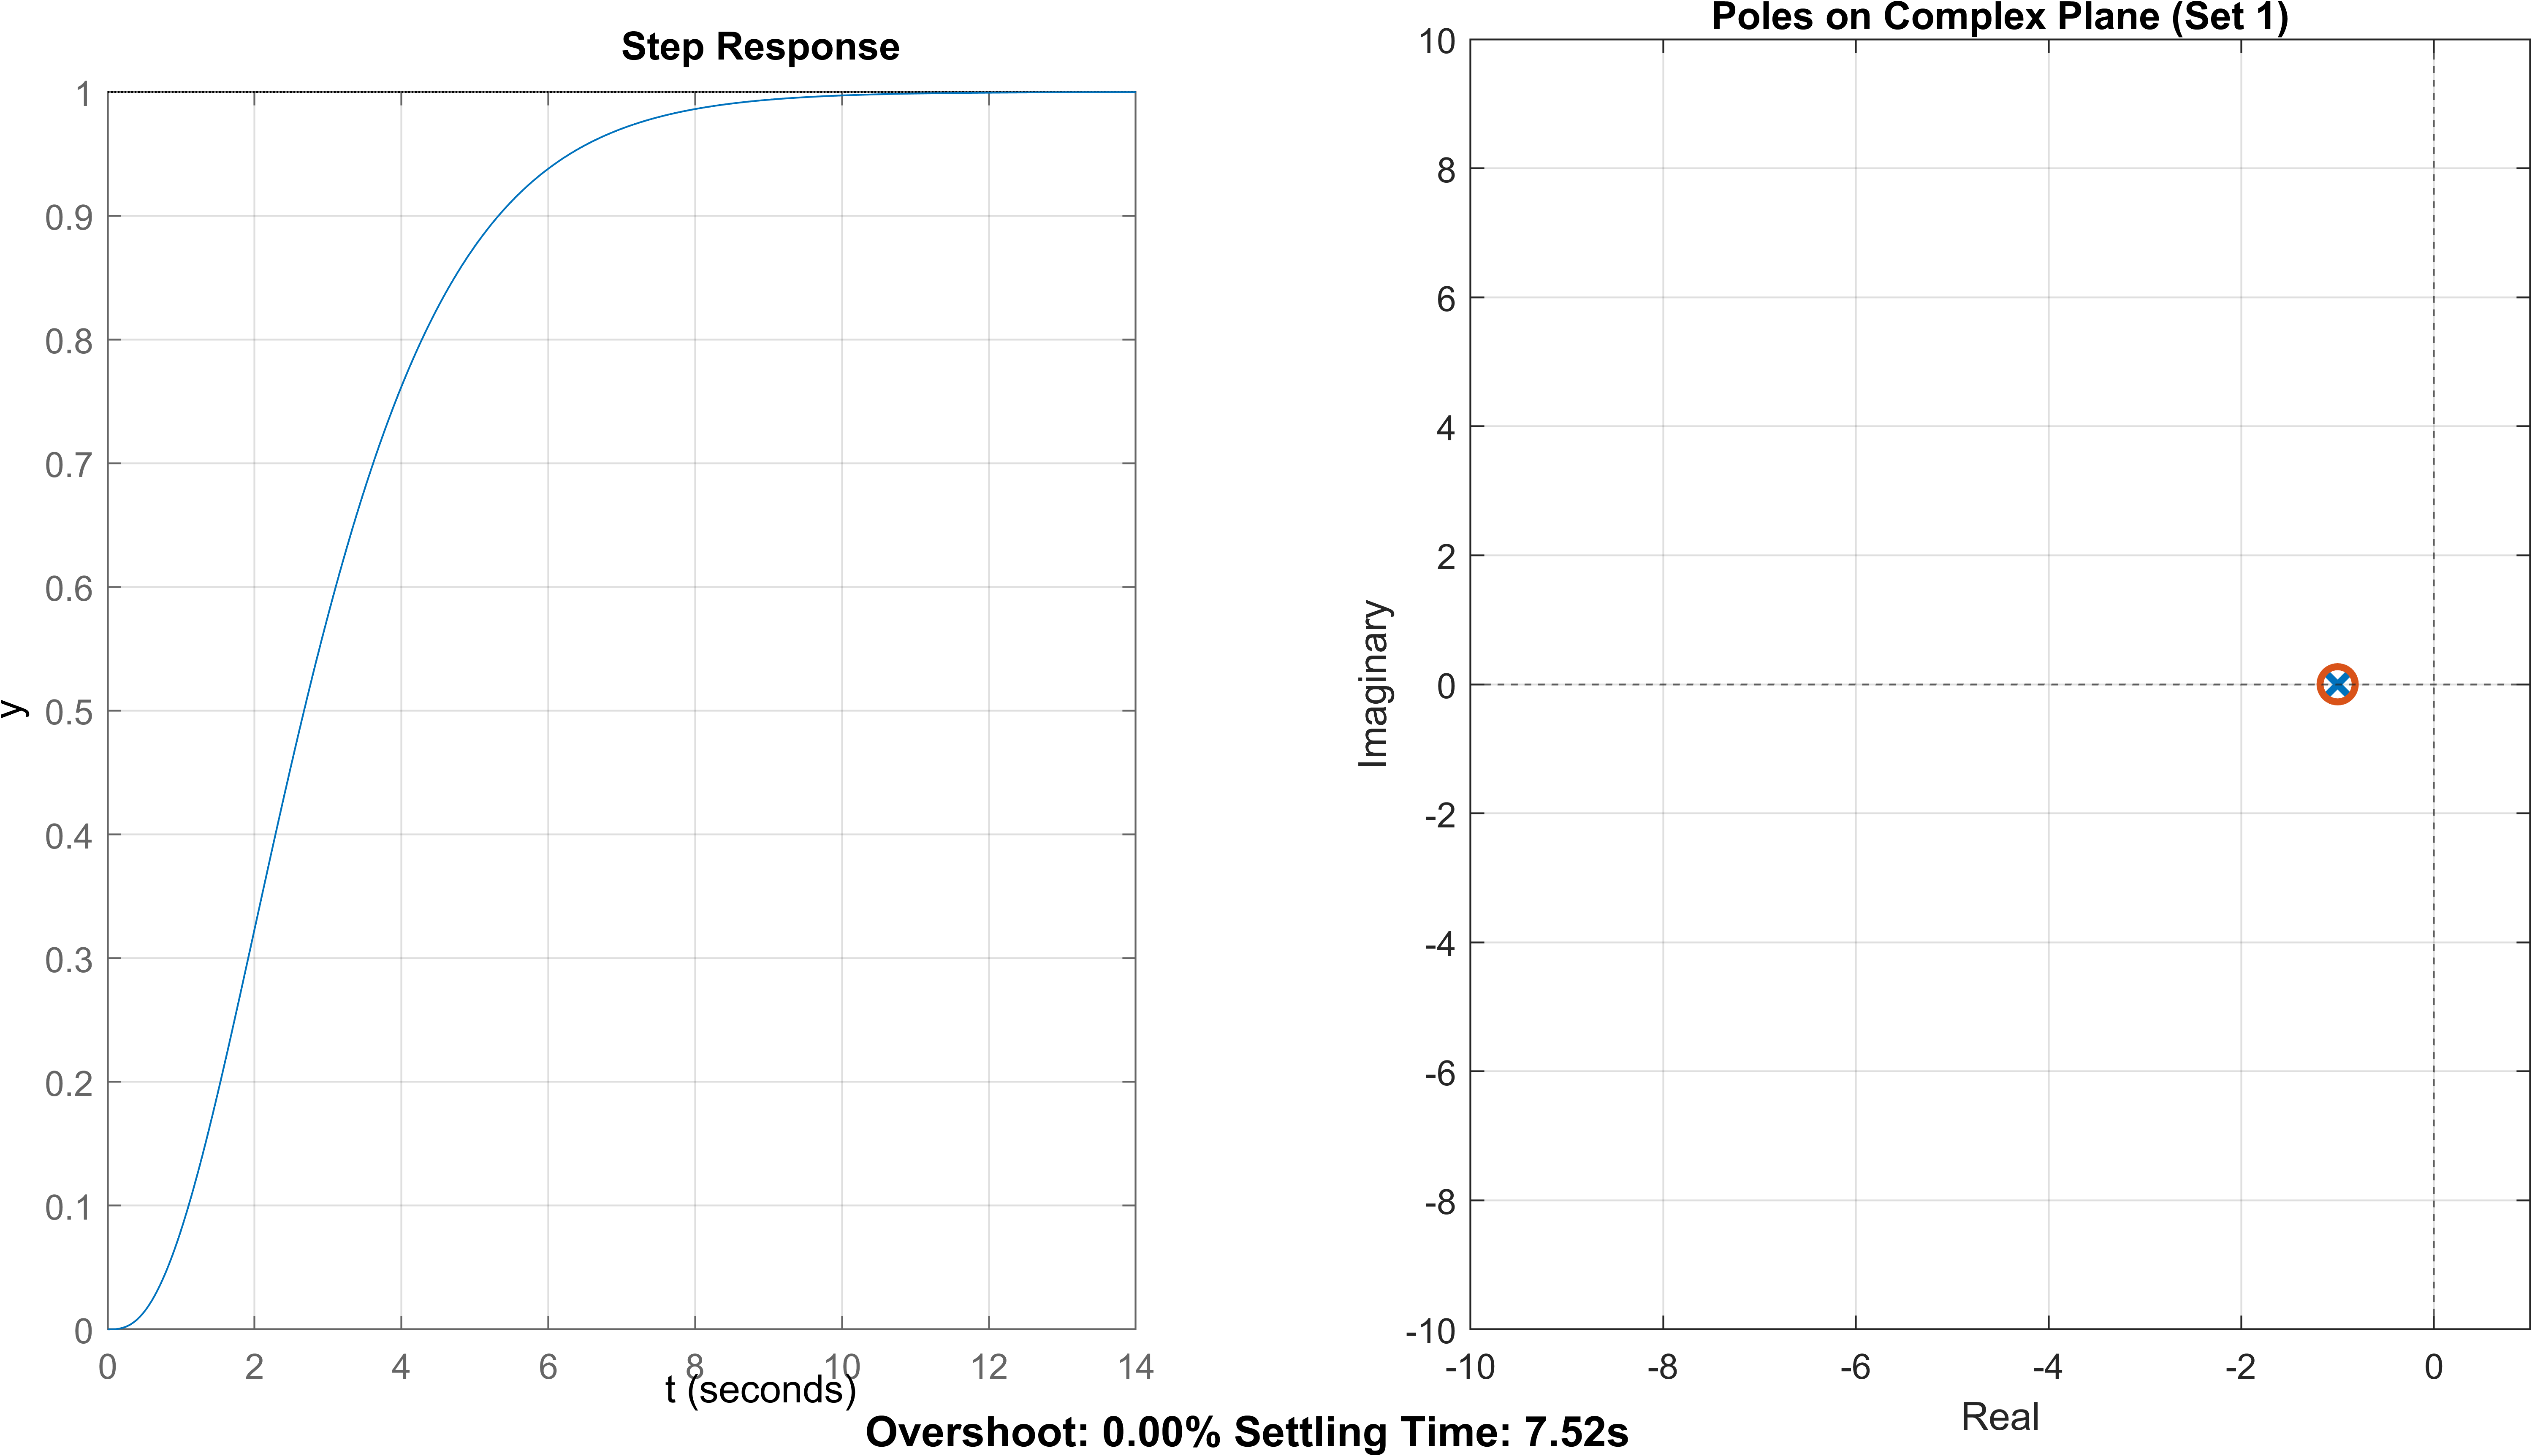
\includegraphics[width=1\textwidth, trim={0cm 0cm 0cm 0cm}]{../images/4_1.png}
    \caption{$\lambda_1 = -1, \lambda_2 = -1, \lambda_3 = -1$}
\end{figure}

\begin{figure}[H]
    \centering
    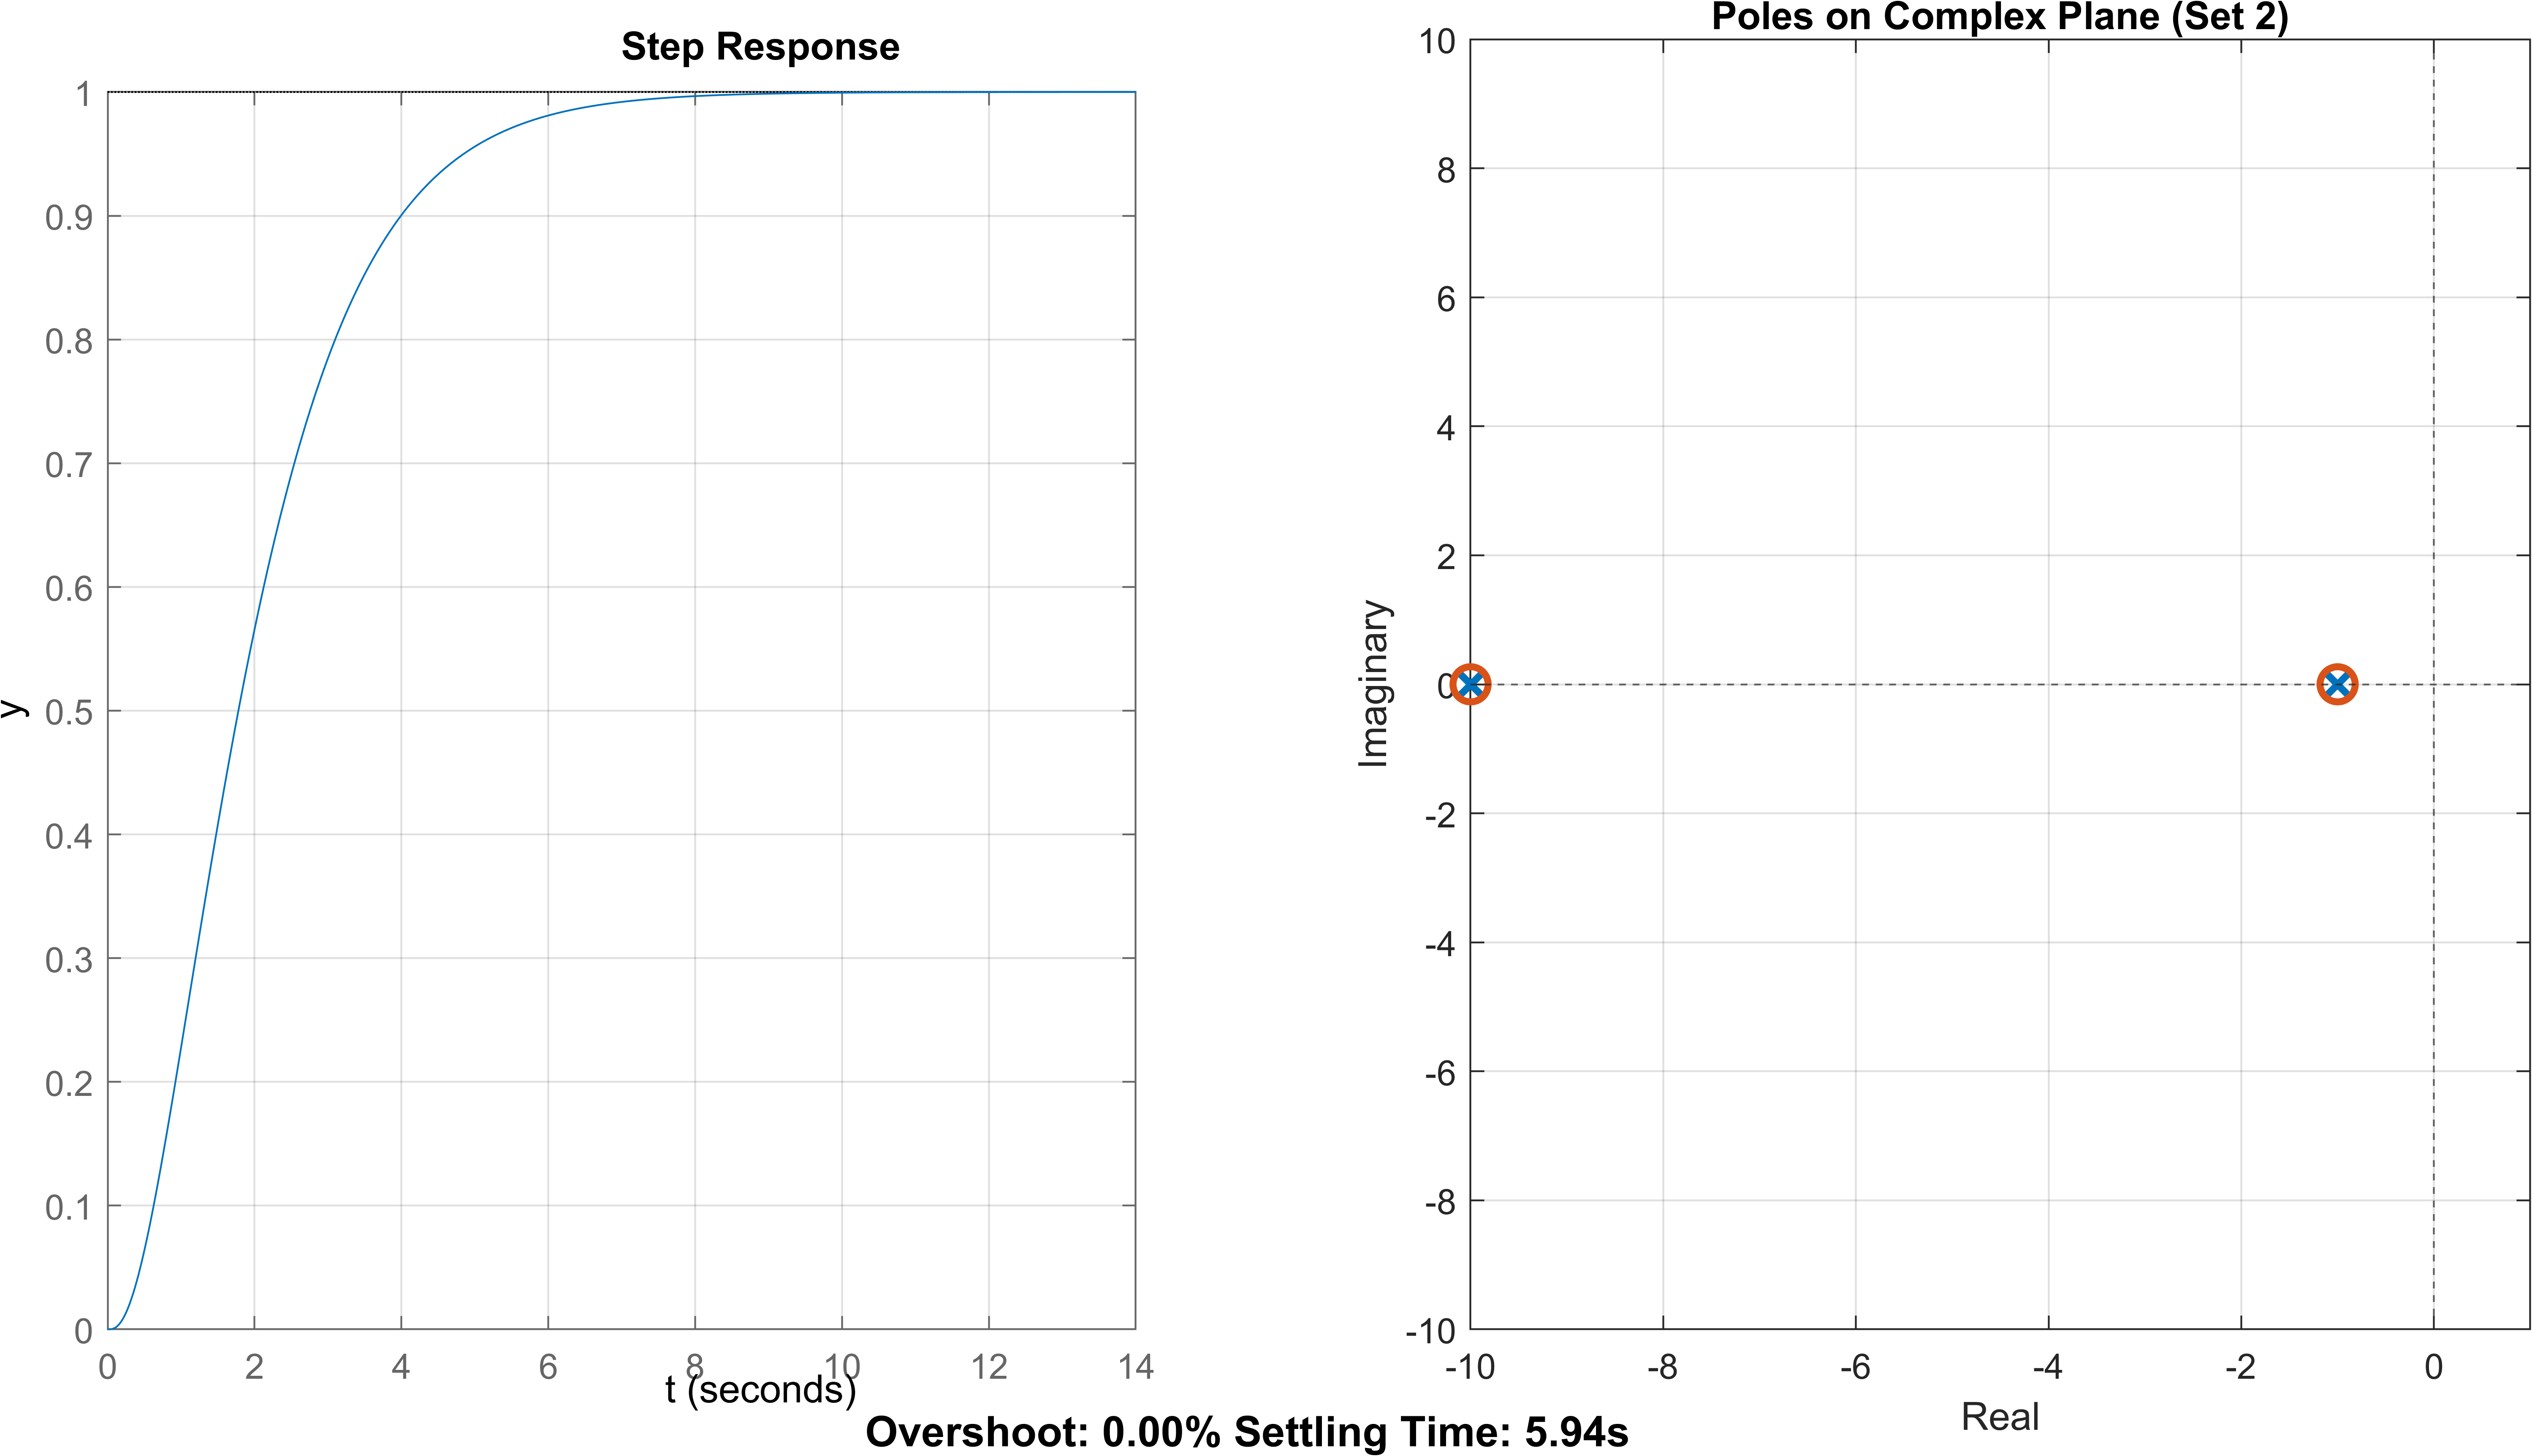
\includegraphics[width=1\textwidth, trim={0cm 0cm 0cm 0cm}]{../images/4_2.png}
    \caption{$\lambda_1 = -1, \lambda_2 = -10, \lambda_3 = -1$}
\end{figure}

\begin{figure}[H]
    \centering
    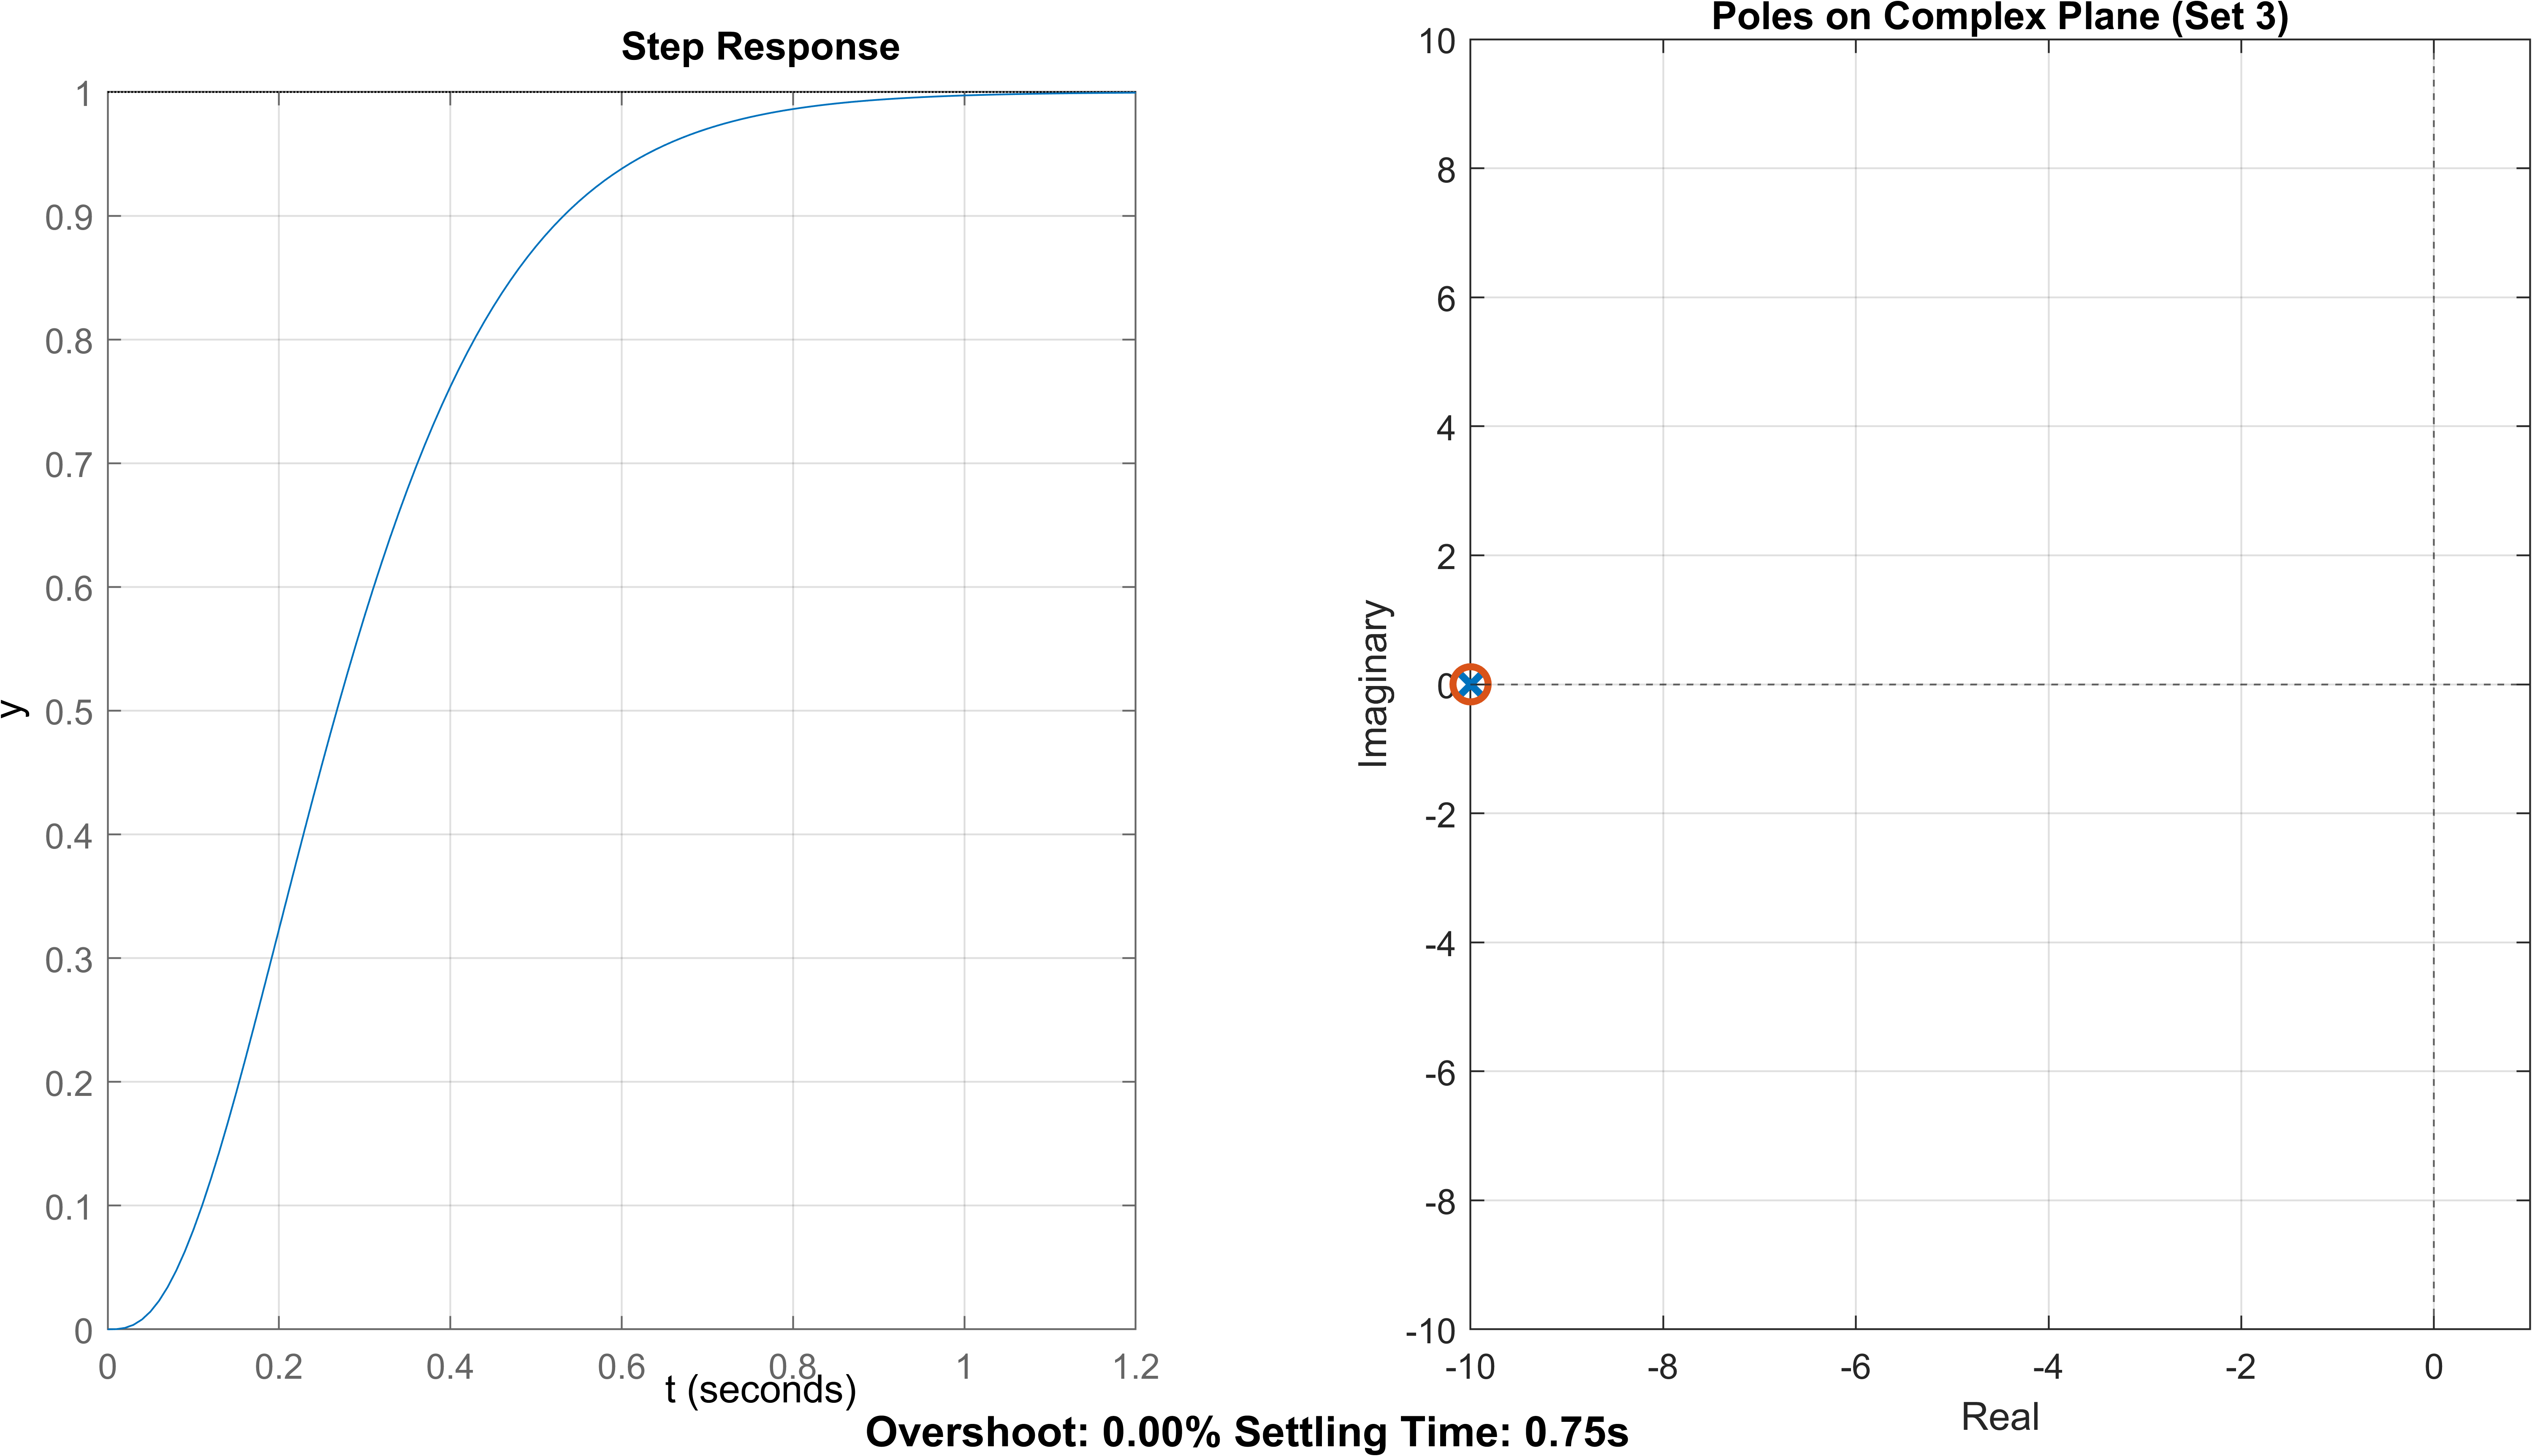
\includegraphics[width=1\textwidth, trim={0cm 0cm 0cm 0cm}]{../images/4_3.png}
    \caption{$\lambda_1 = -10, \lambda_2 = -10, \lambda_3 = -10$}
\end{figure}

\begin{figure}[H]
    \centering
    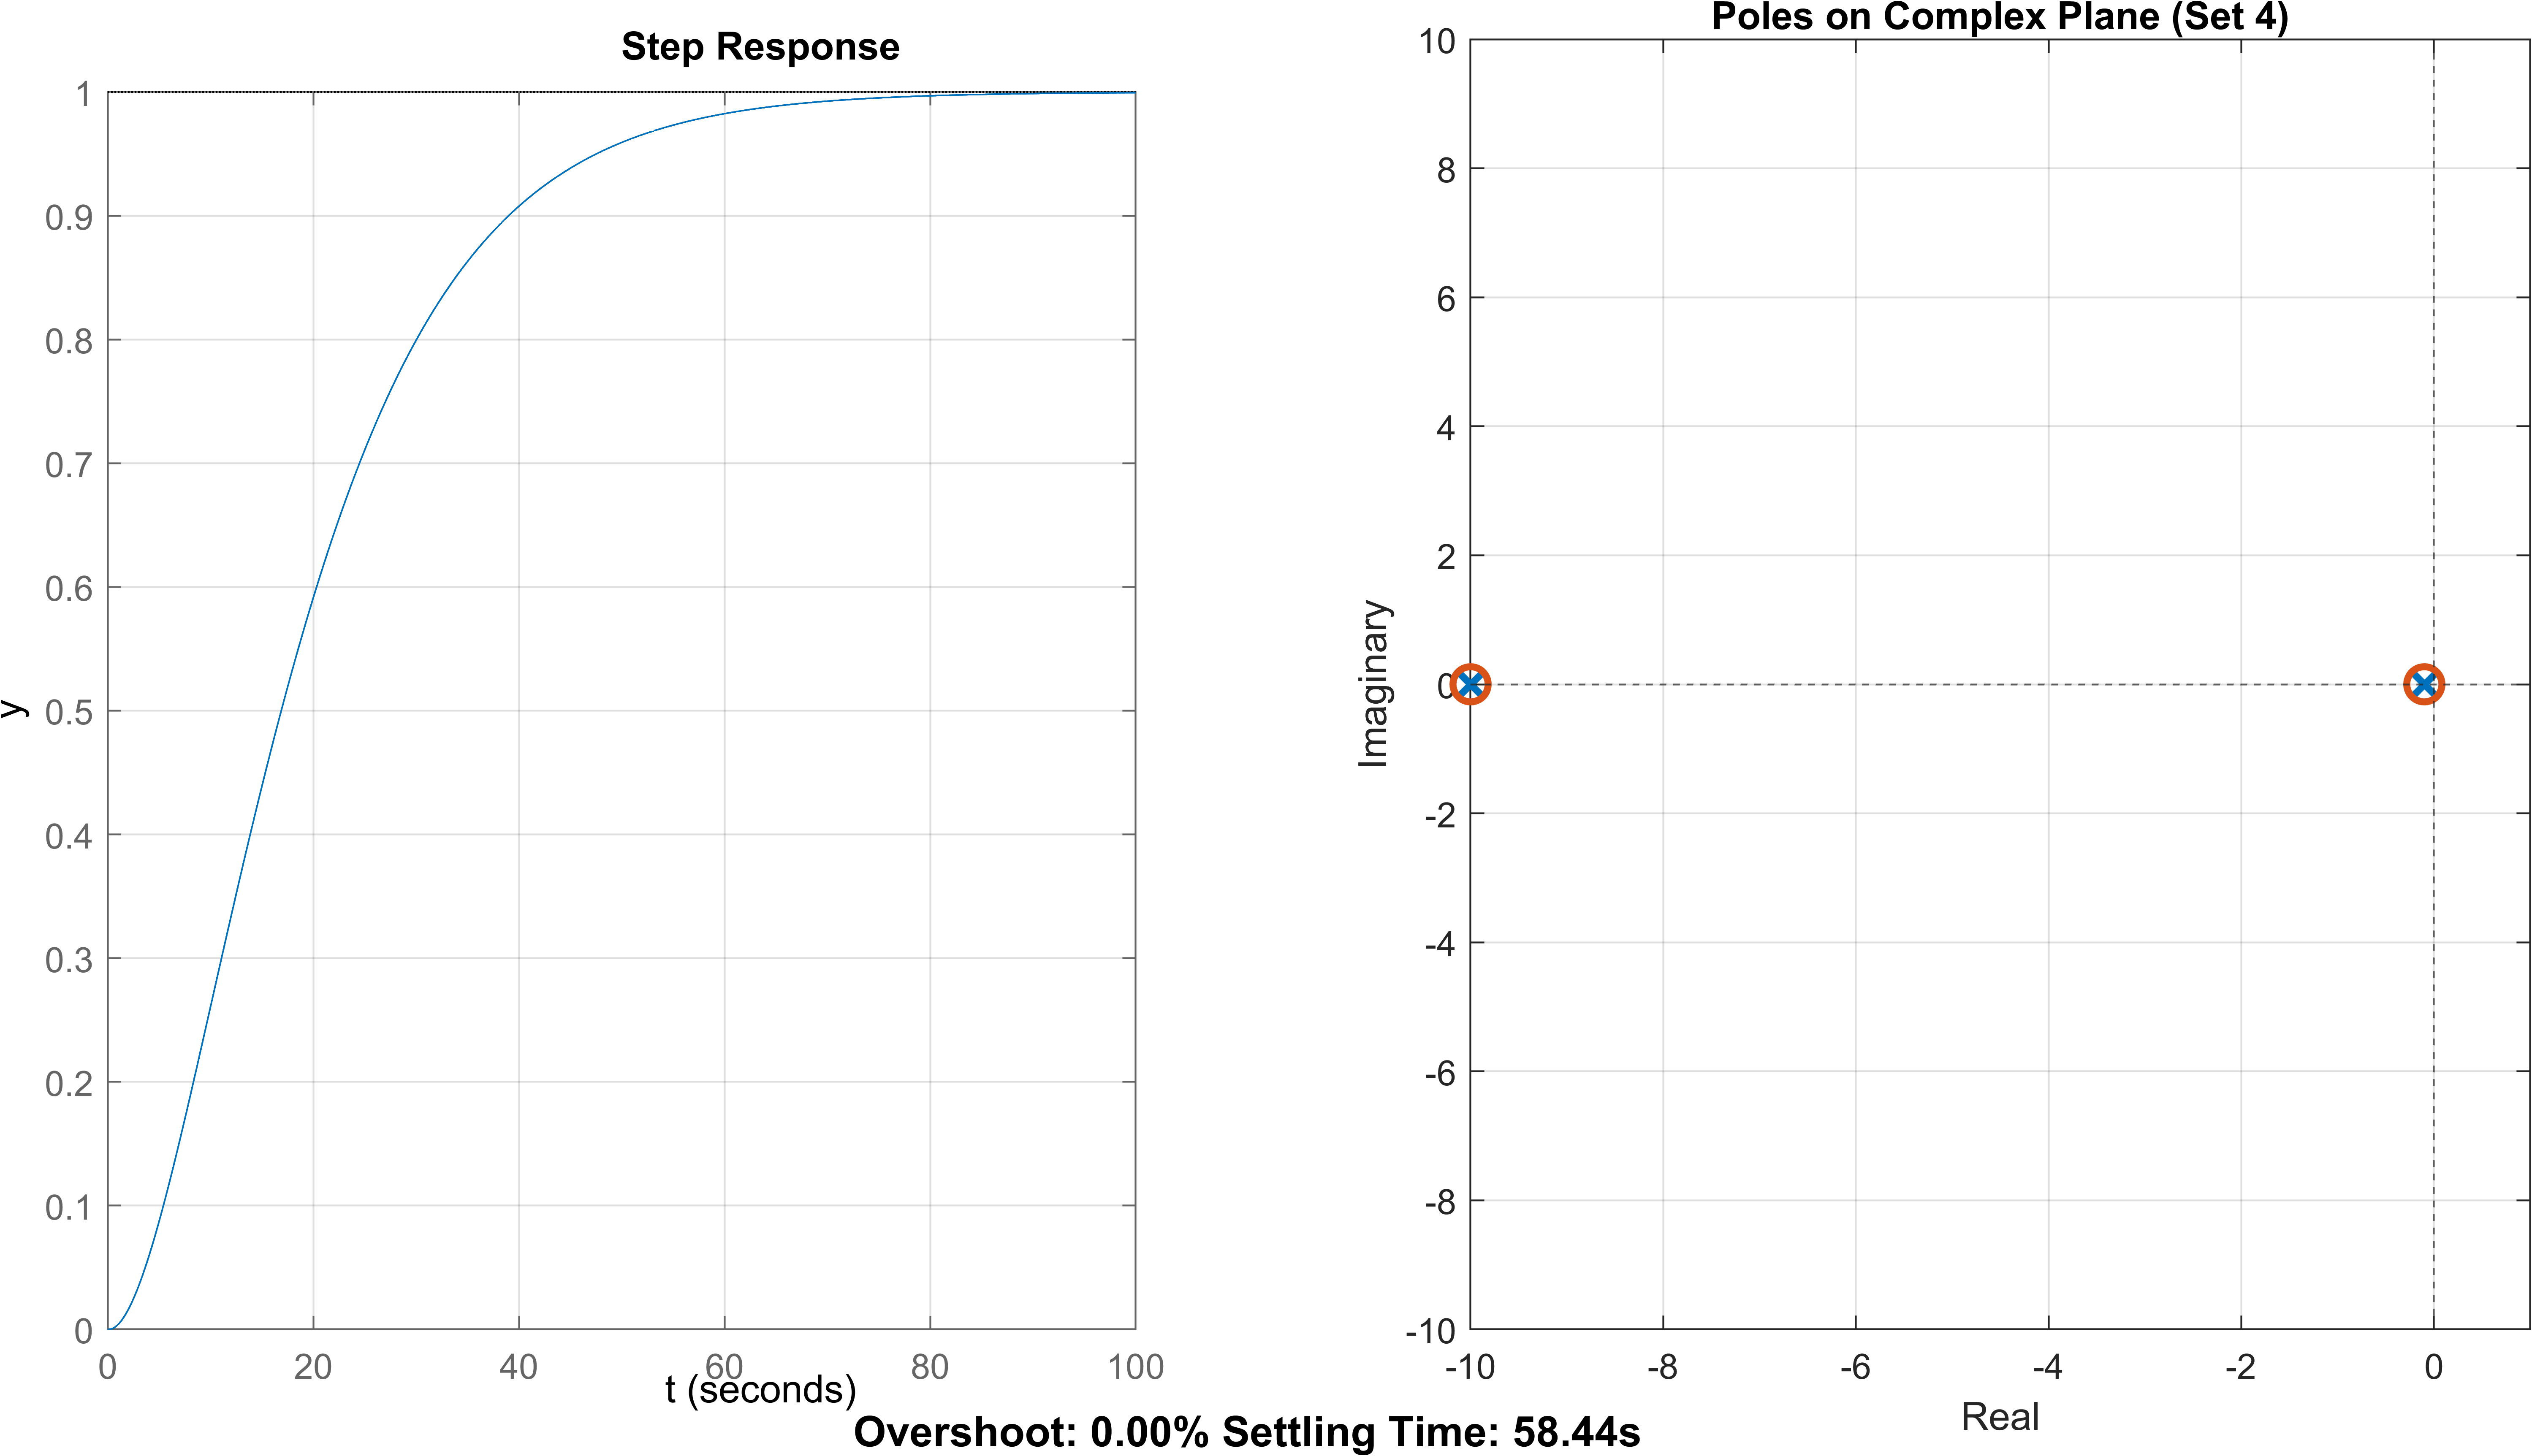
\includegraphics[width=1\textwidth, trim={0cm 0cm 0cm 0cm}]{../images/4_4.png}
    \caption{$\lambda_1 = -0.1, \lambda_2 = -10, \lambda_3 = -0.1$}
\end{figure}

\begin{figure}[H]
    \centering
    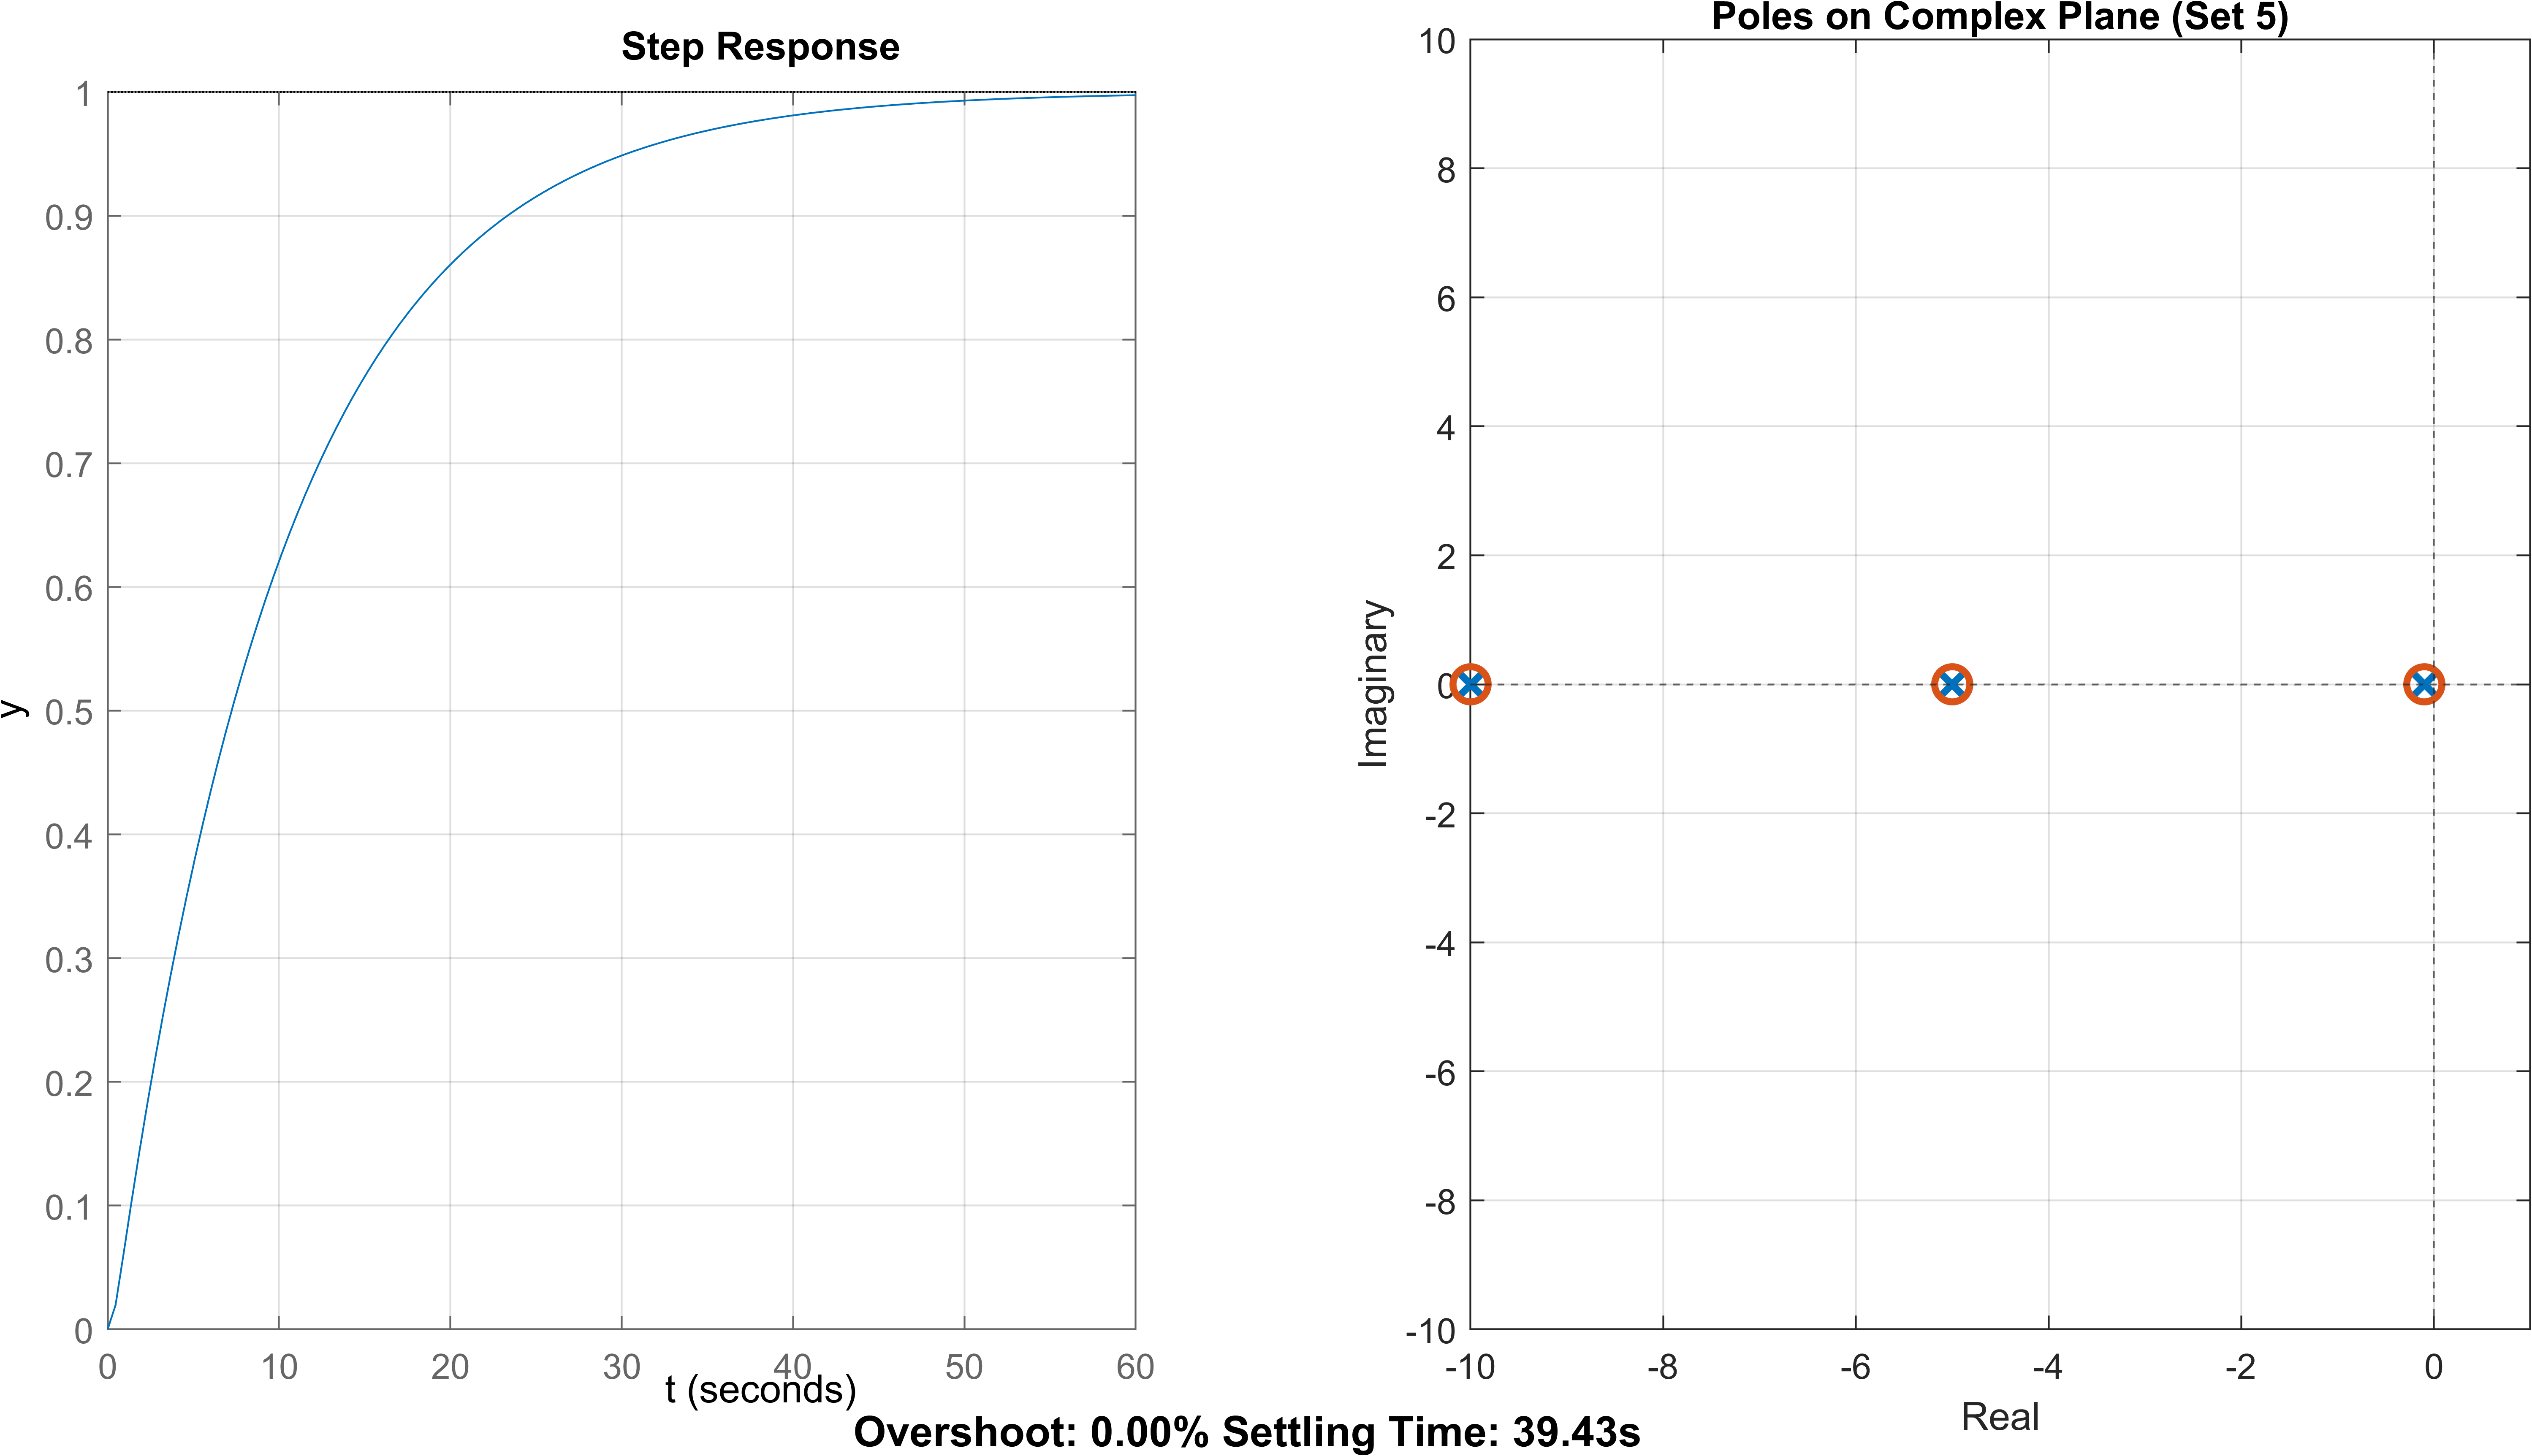
\includegraphics[width=1\textwidth, trim={0cm 0cm 0cm 0cm}]{../images/4_5.png}
    \caption{$\lambda_1 = -0.1, \lambda_2 = -5, \lambda_3 = -10$}
\end{figure}

\begin{figure}[H]
    \centering
    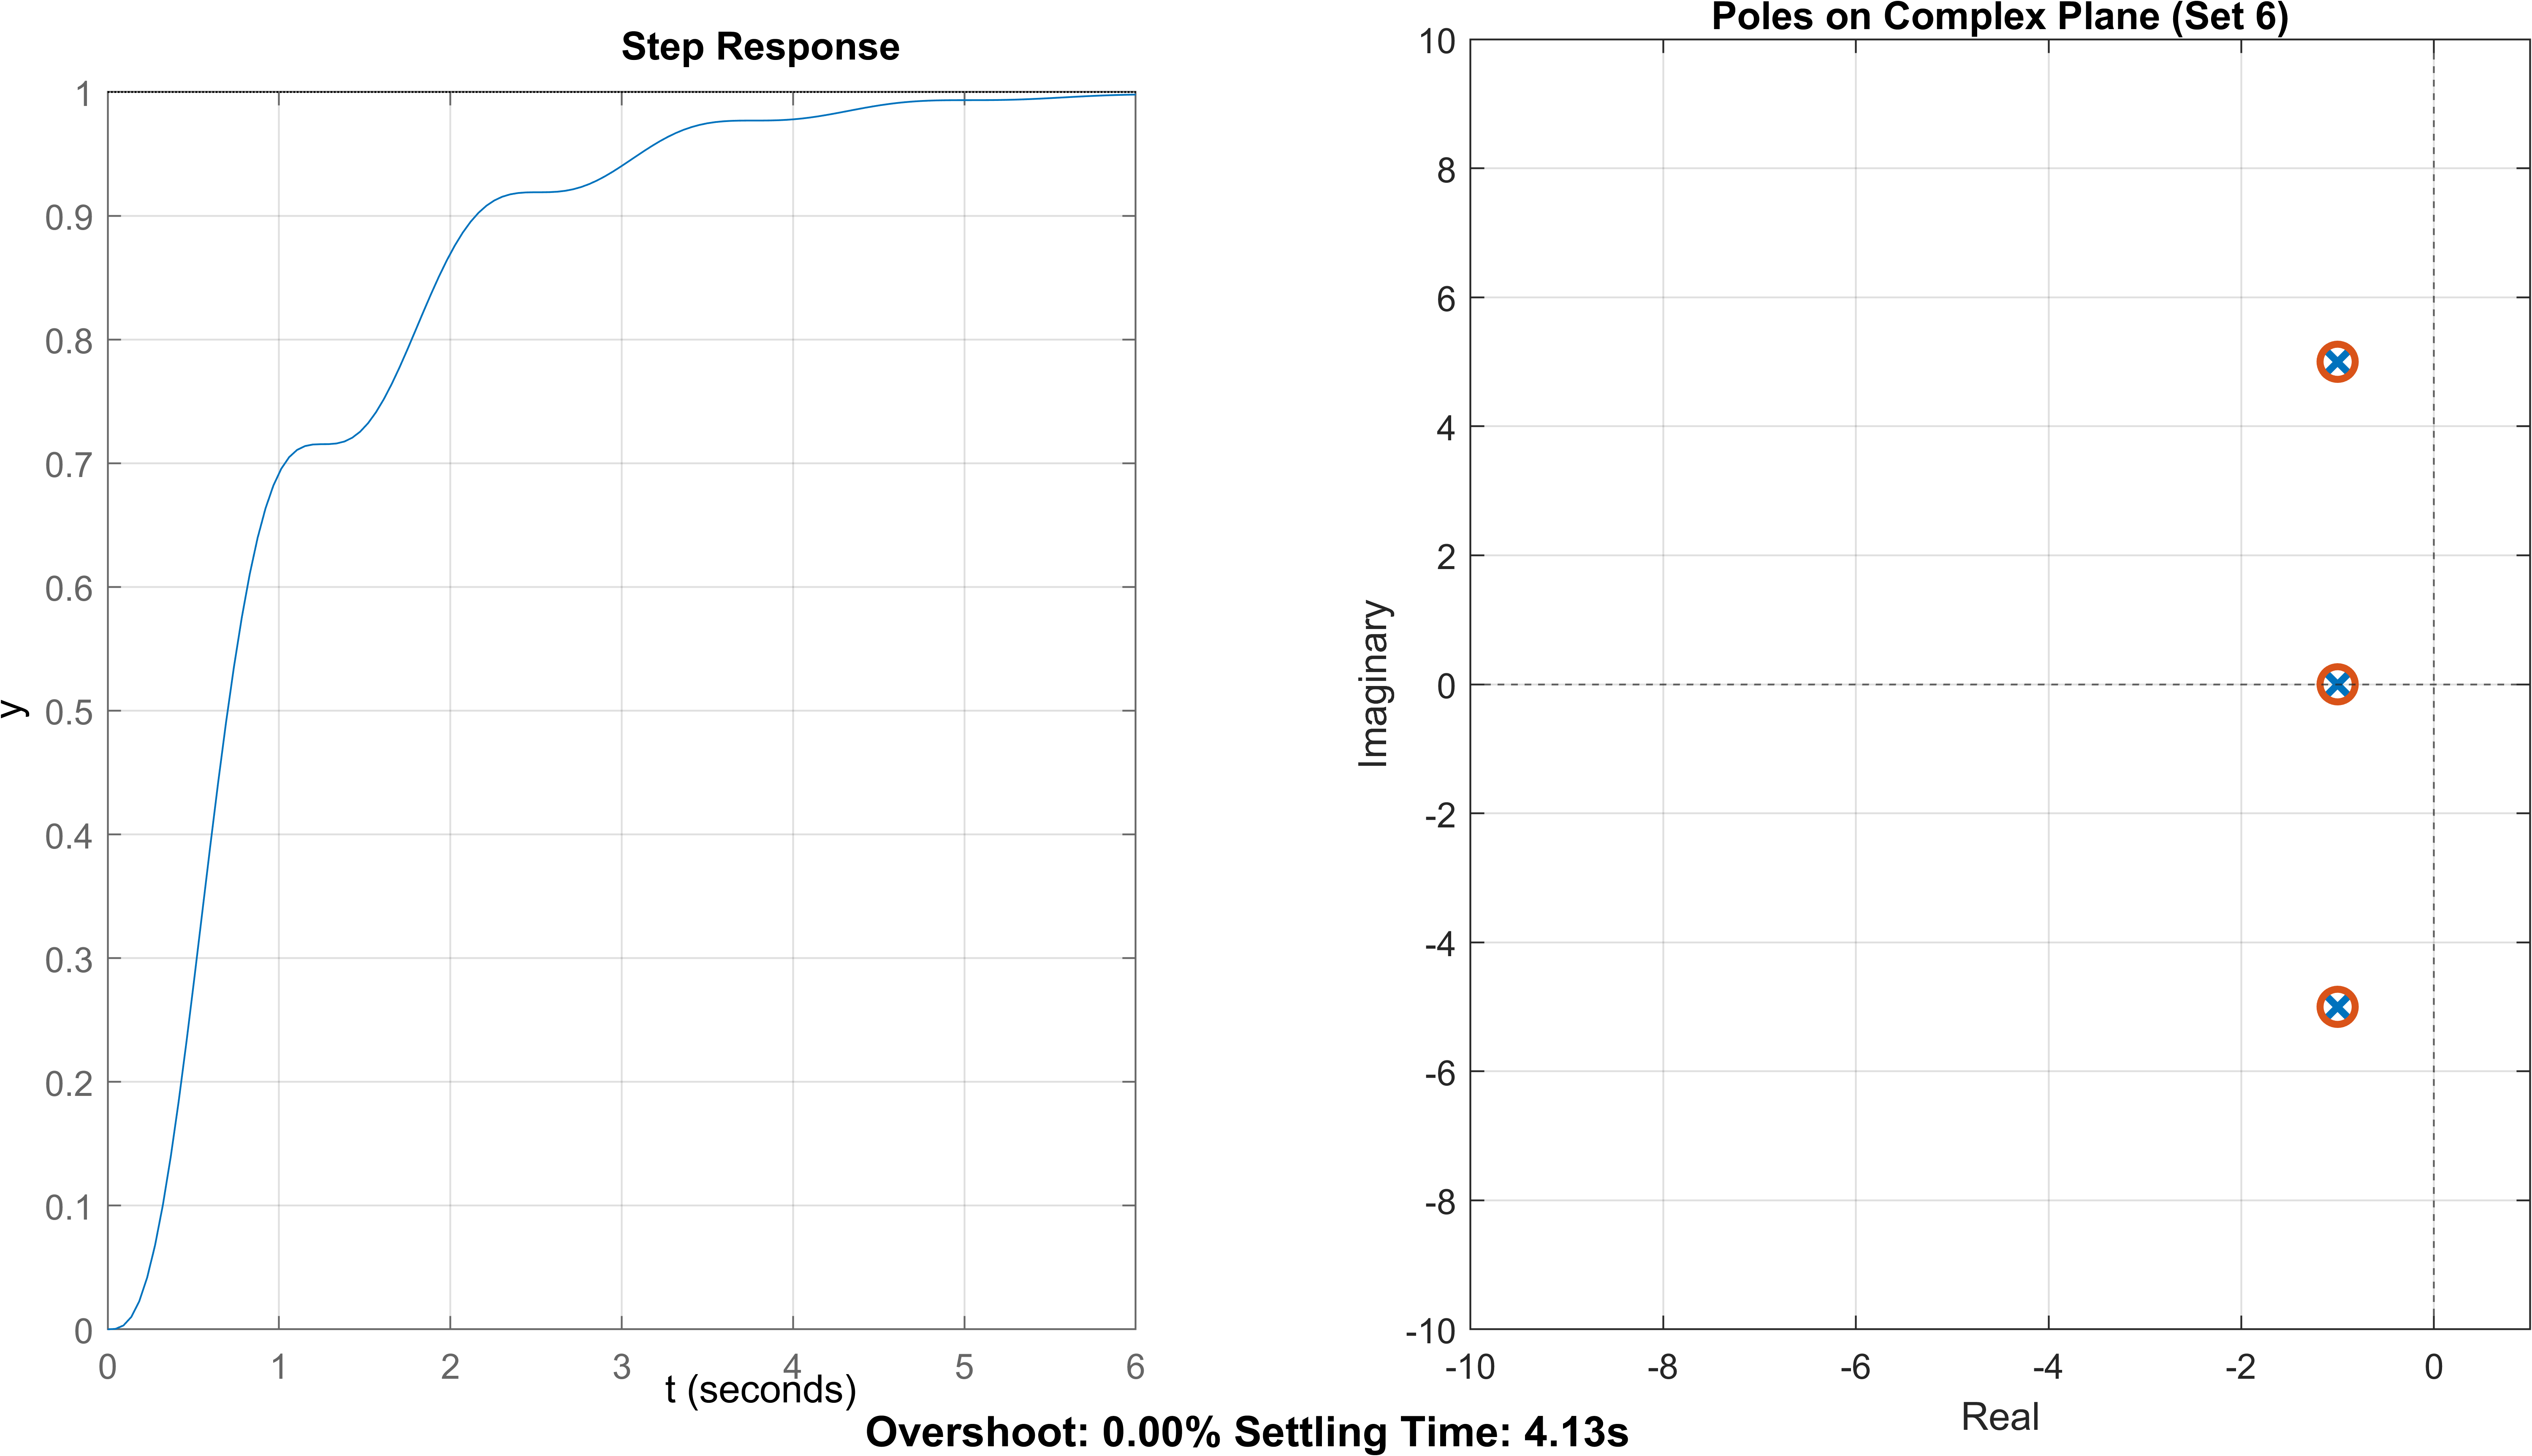
\includegraphics[width=1\textwidth, trim={0cm 0cm 0cm 0cm}]{../images/4_6.png}
    \caption{$\lambda_1 = -1+5i, \lambda_2 = -1-5i, \lambda_3 = -1$}
\end{figure}

\begin{figure}[H]
    \centering
    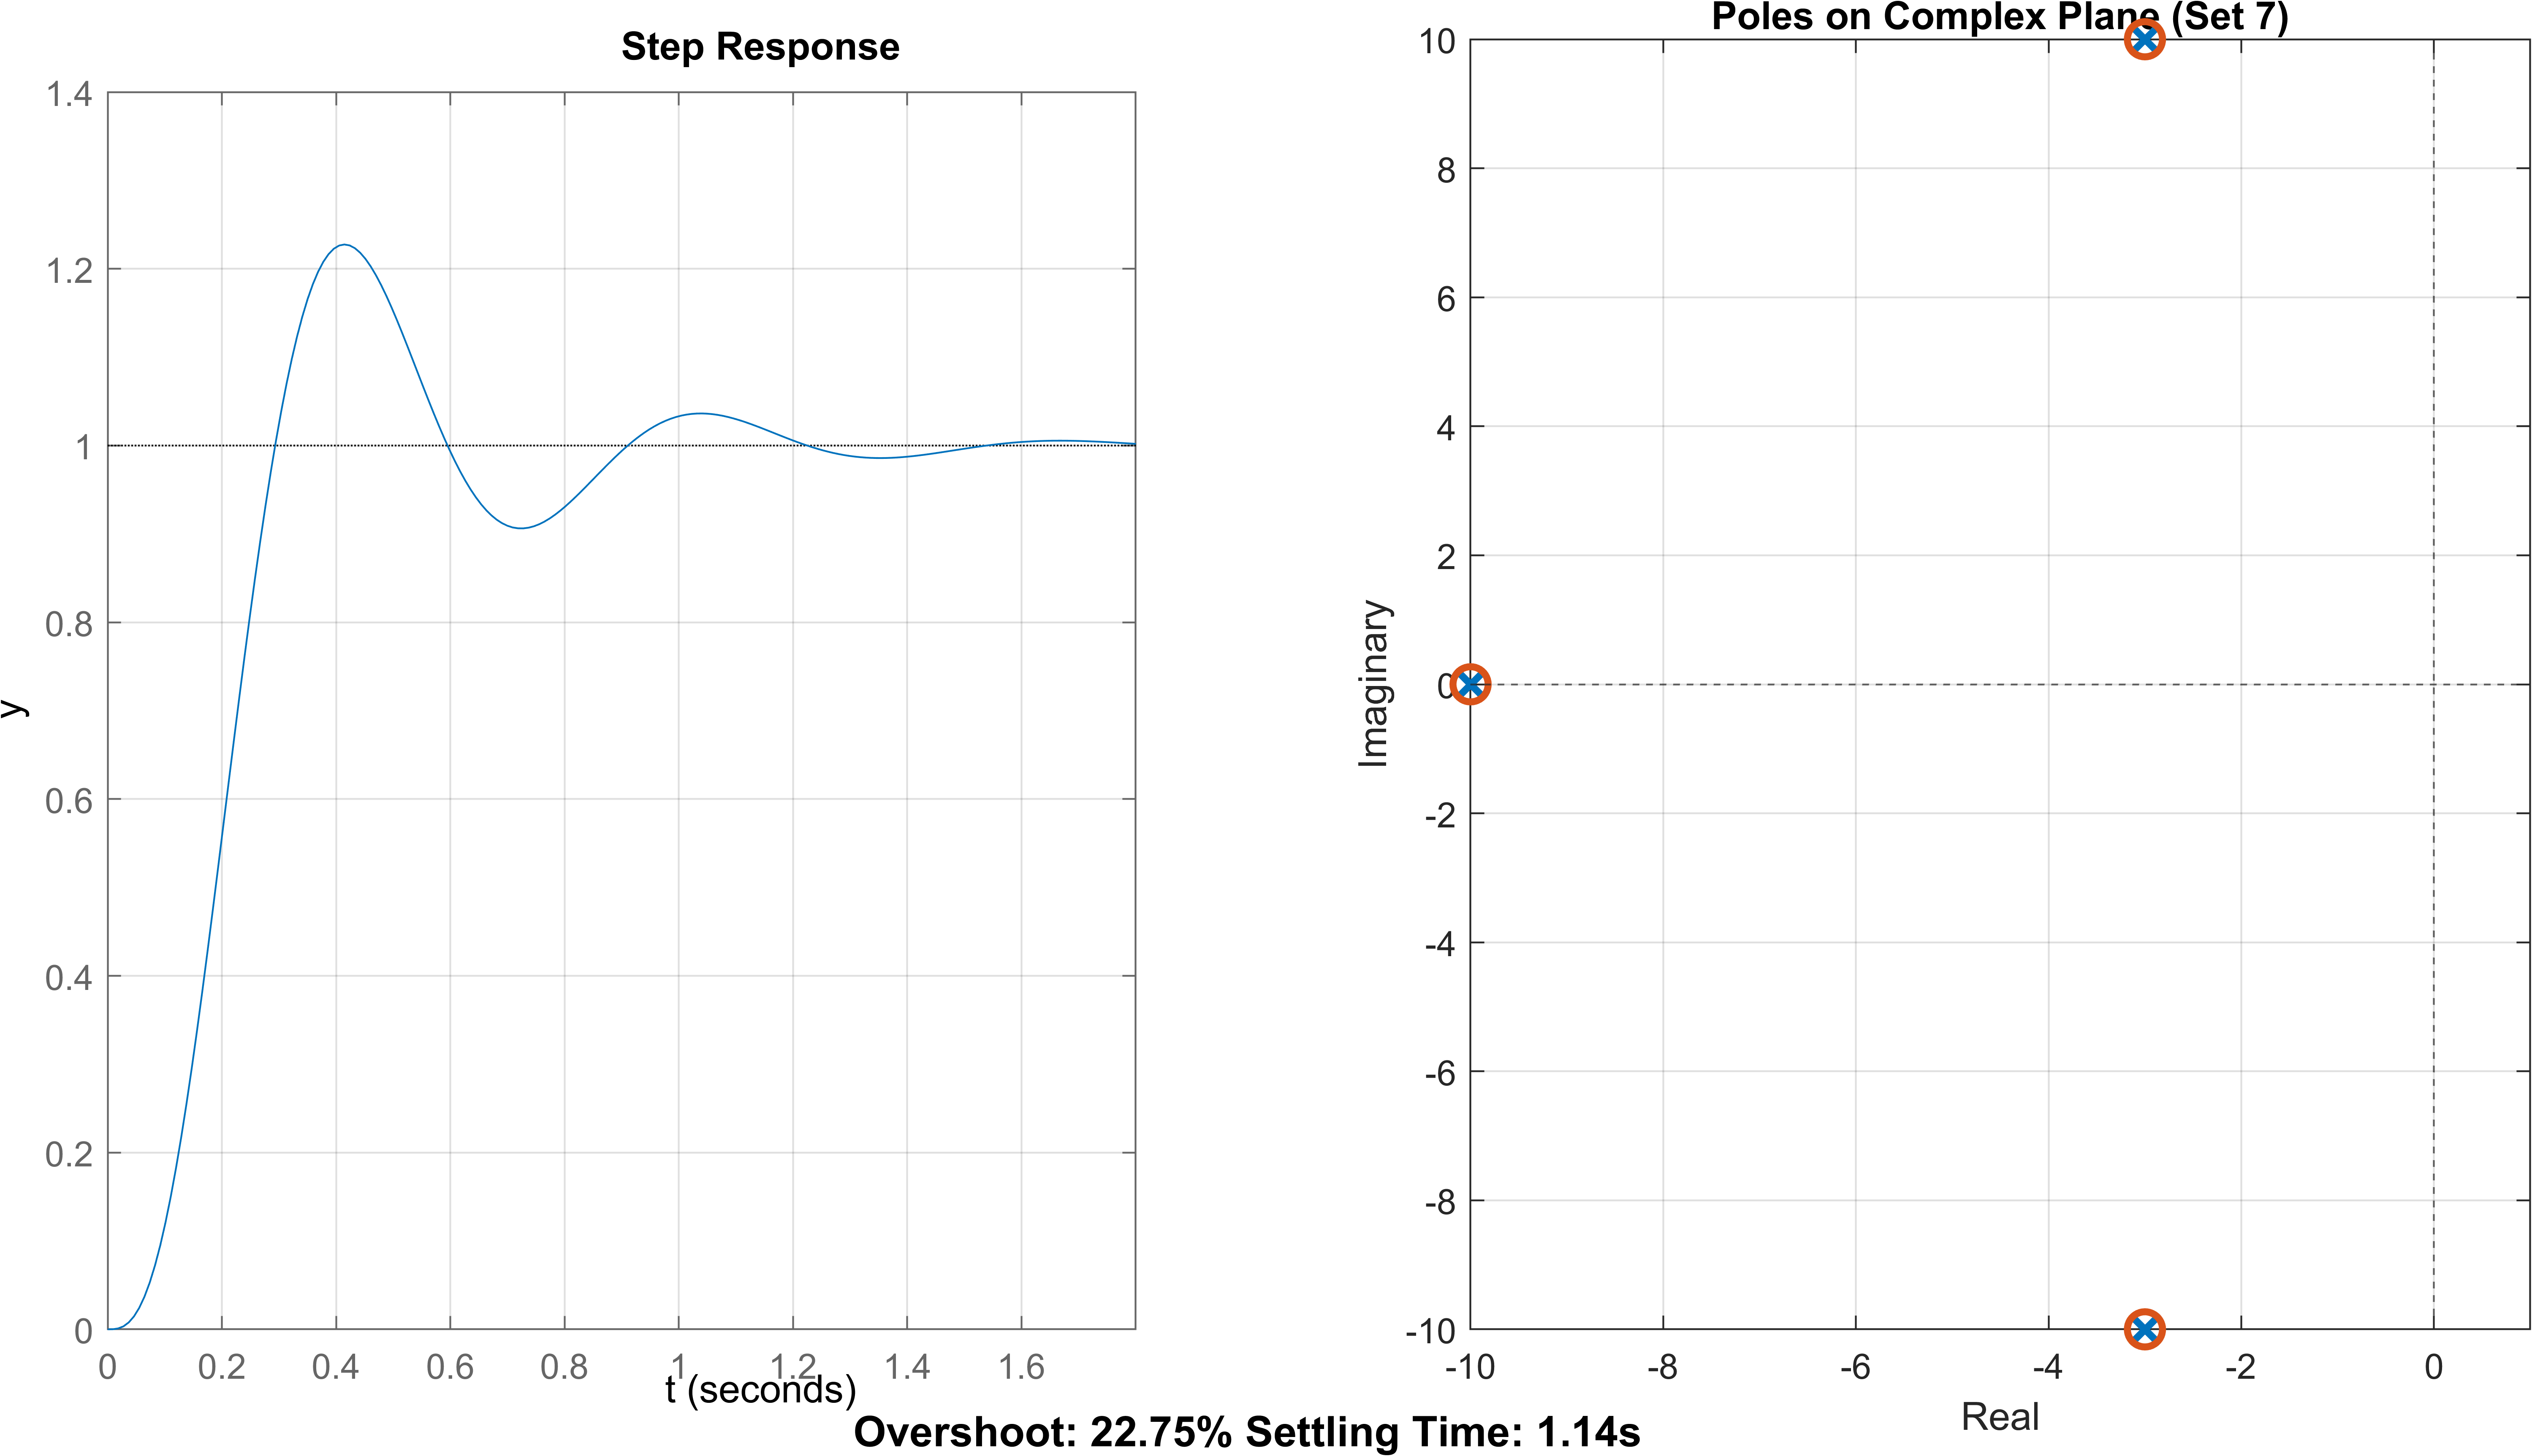
\includegraphics[width=1\textwidth, trim={0cm 0cm 0cm 0cm}]{../images/4_7.png}
    \caption{$\lambda_1 = -3+10i, \lambda_2 = -3-10i, \lambda_3 = -10$}
\end{figure}

\begin{figure}[H]
    \centering
    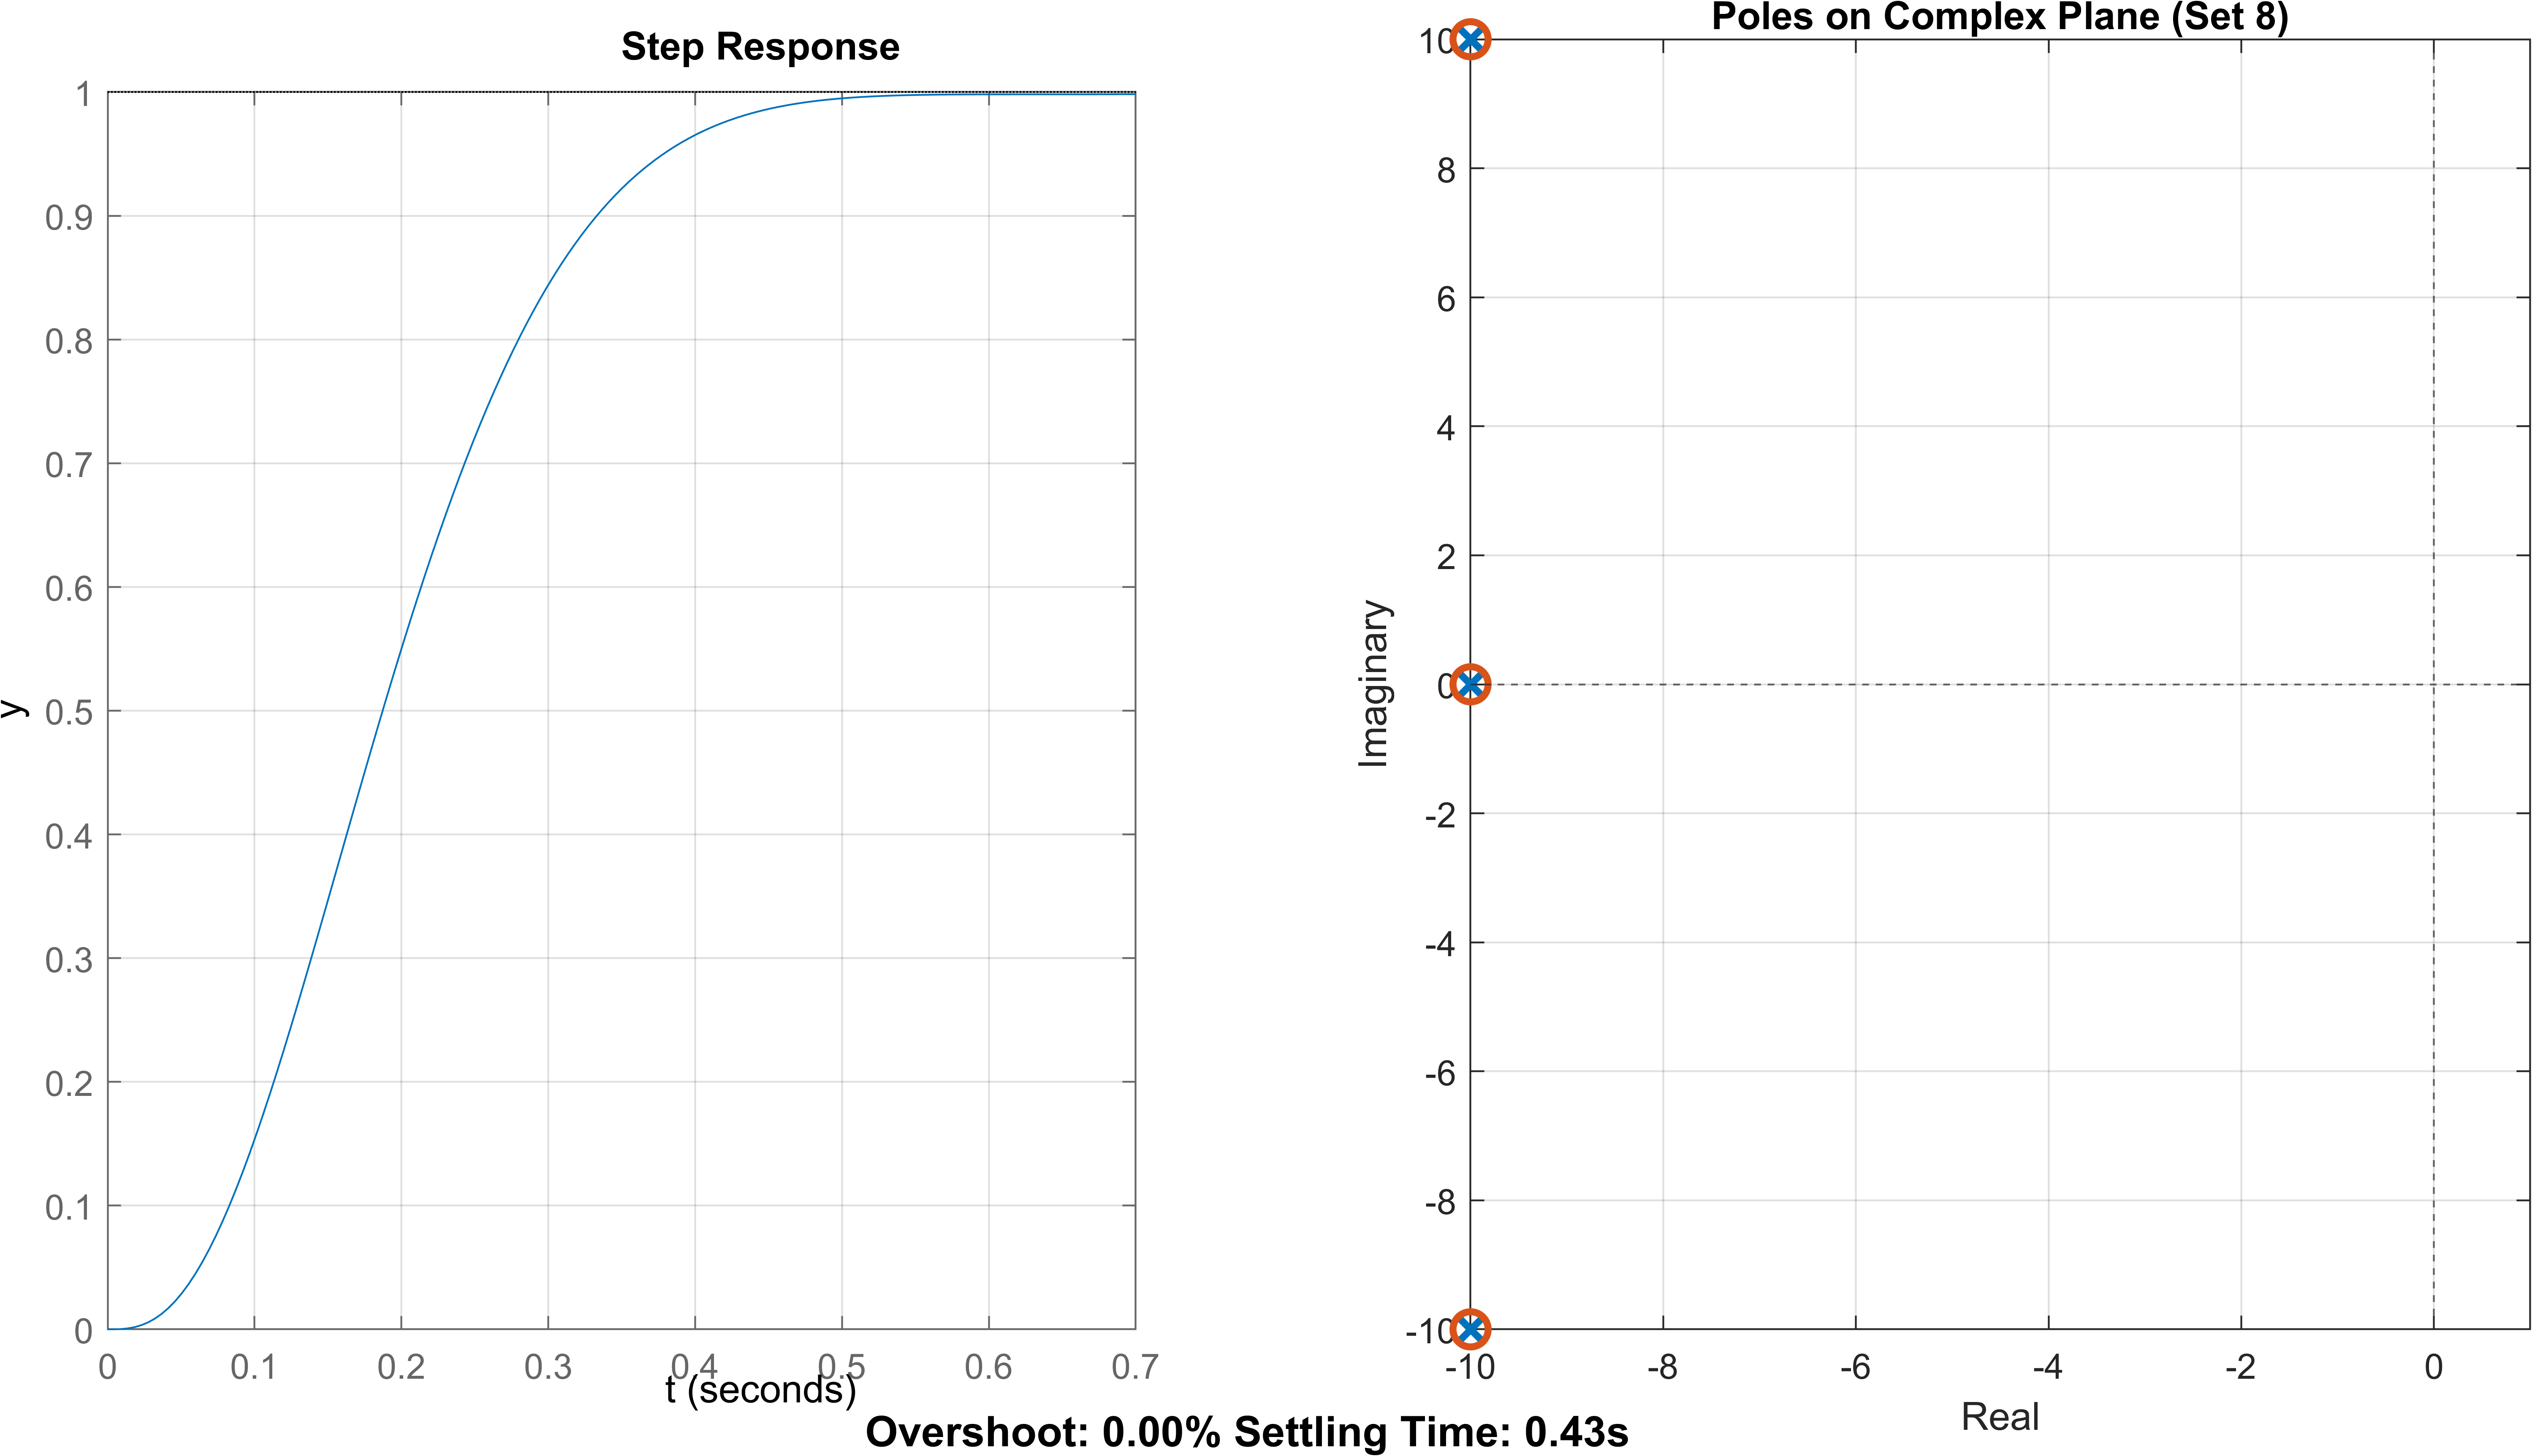
\includegraphics[width=1\textwidth, trim={0cm 0cm 0cm 0cm}]{../images/4_8.png}
    \caption{$\lambda_1 = -10 + 10i, \lambda_2 = -10 - 10i, \lambda_3 = -10$}
\end{figure}

\begin{figure}[H]
    \centering
    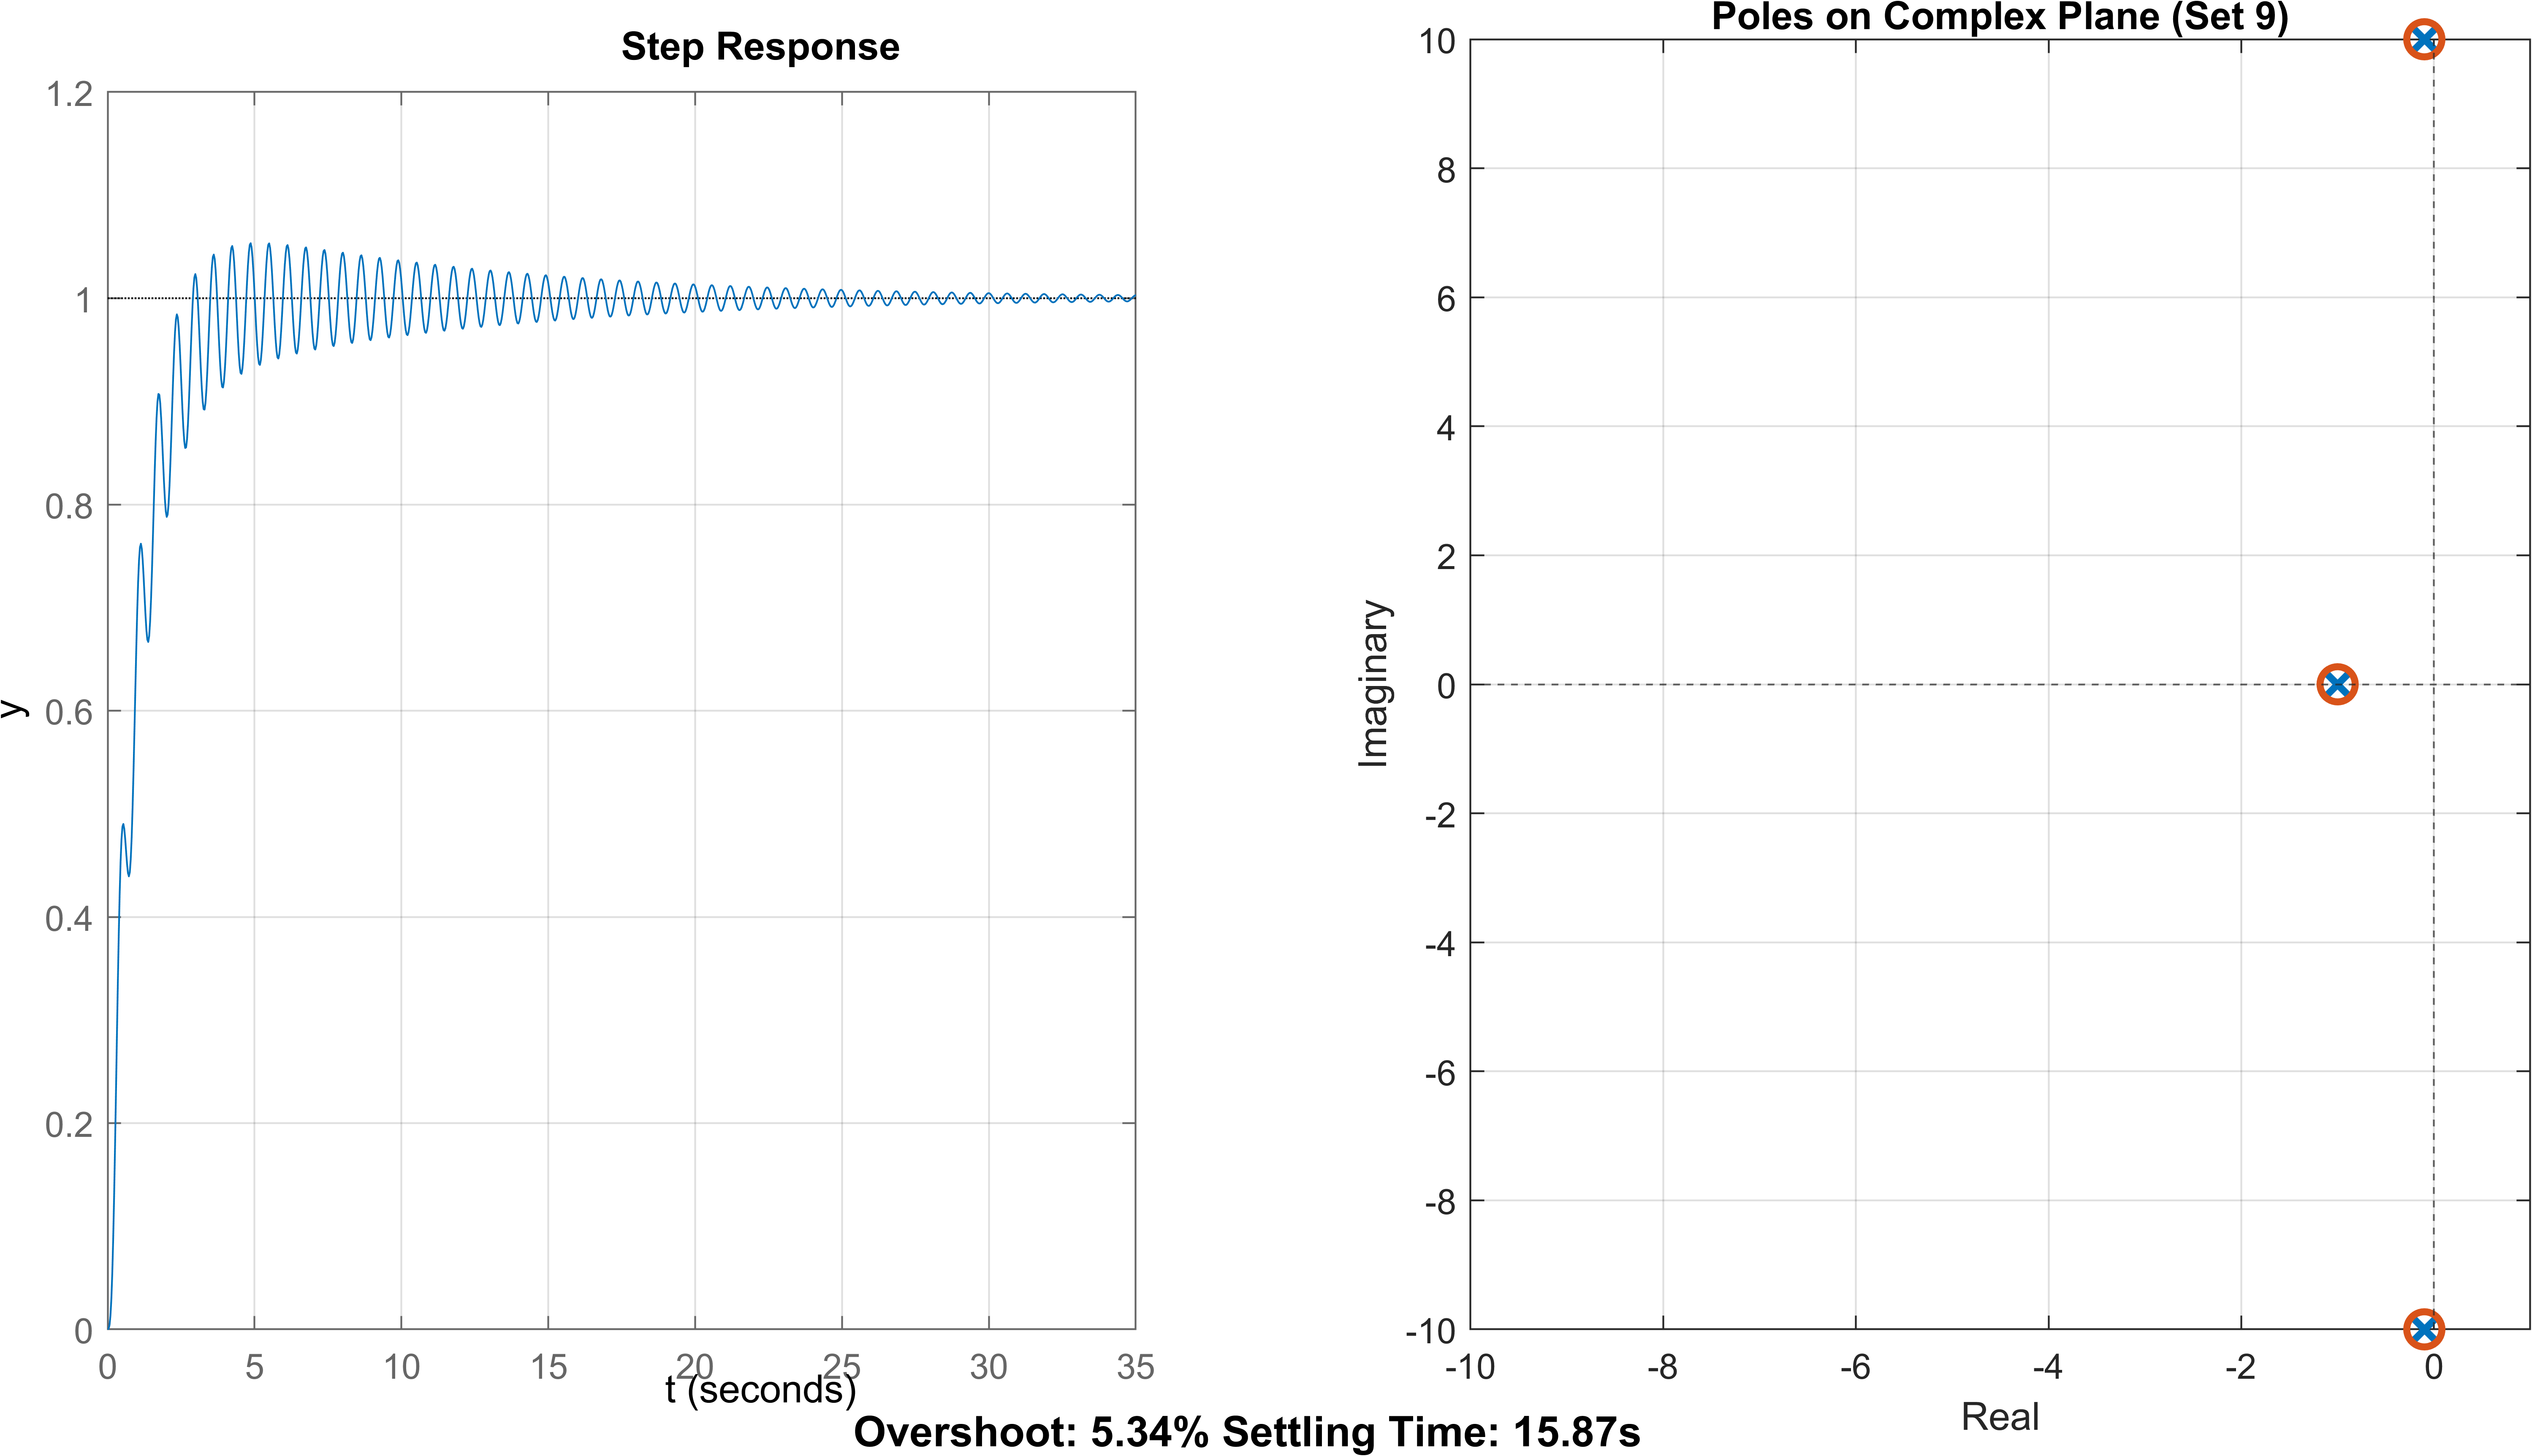
\includegraphics[width=1\textwidth, trim={0cm 0cm 0cm 0cm}]{../images/4_9.png}
    \caption{$\lambda_1 = -0.1+ 10i, \lambda_2 = -0.1 - 10i, \lambda_3 = -1$}
\end{figure}

\begin{figure}[H]
    \centering
    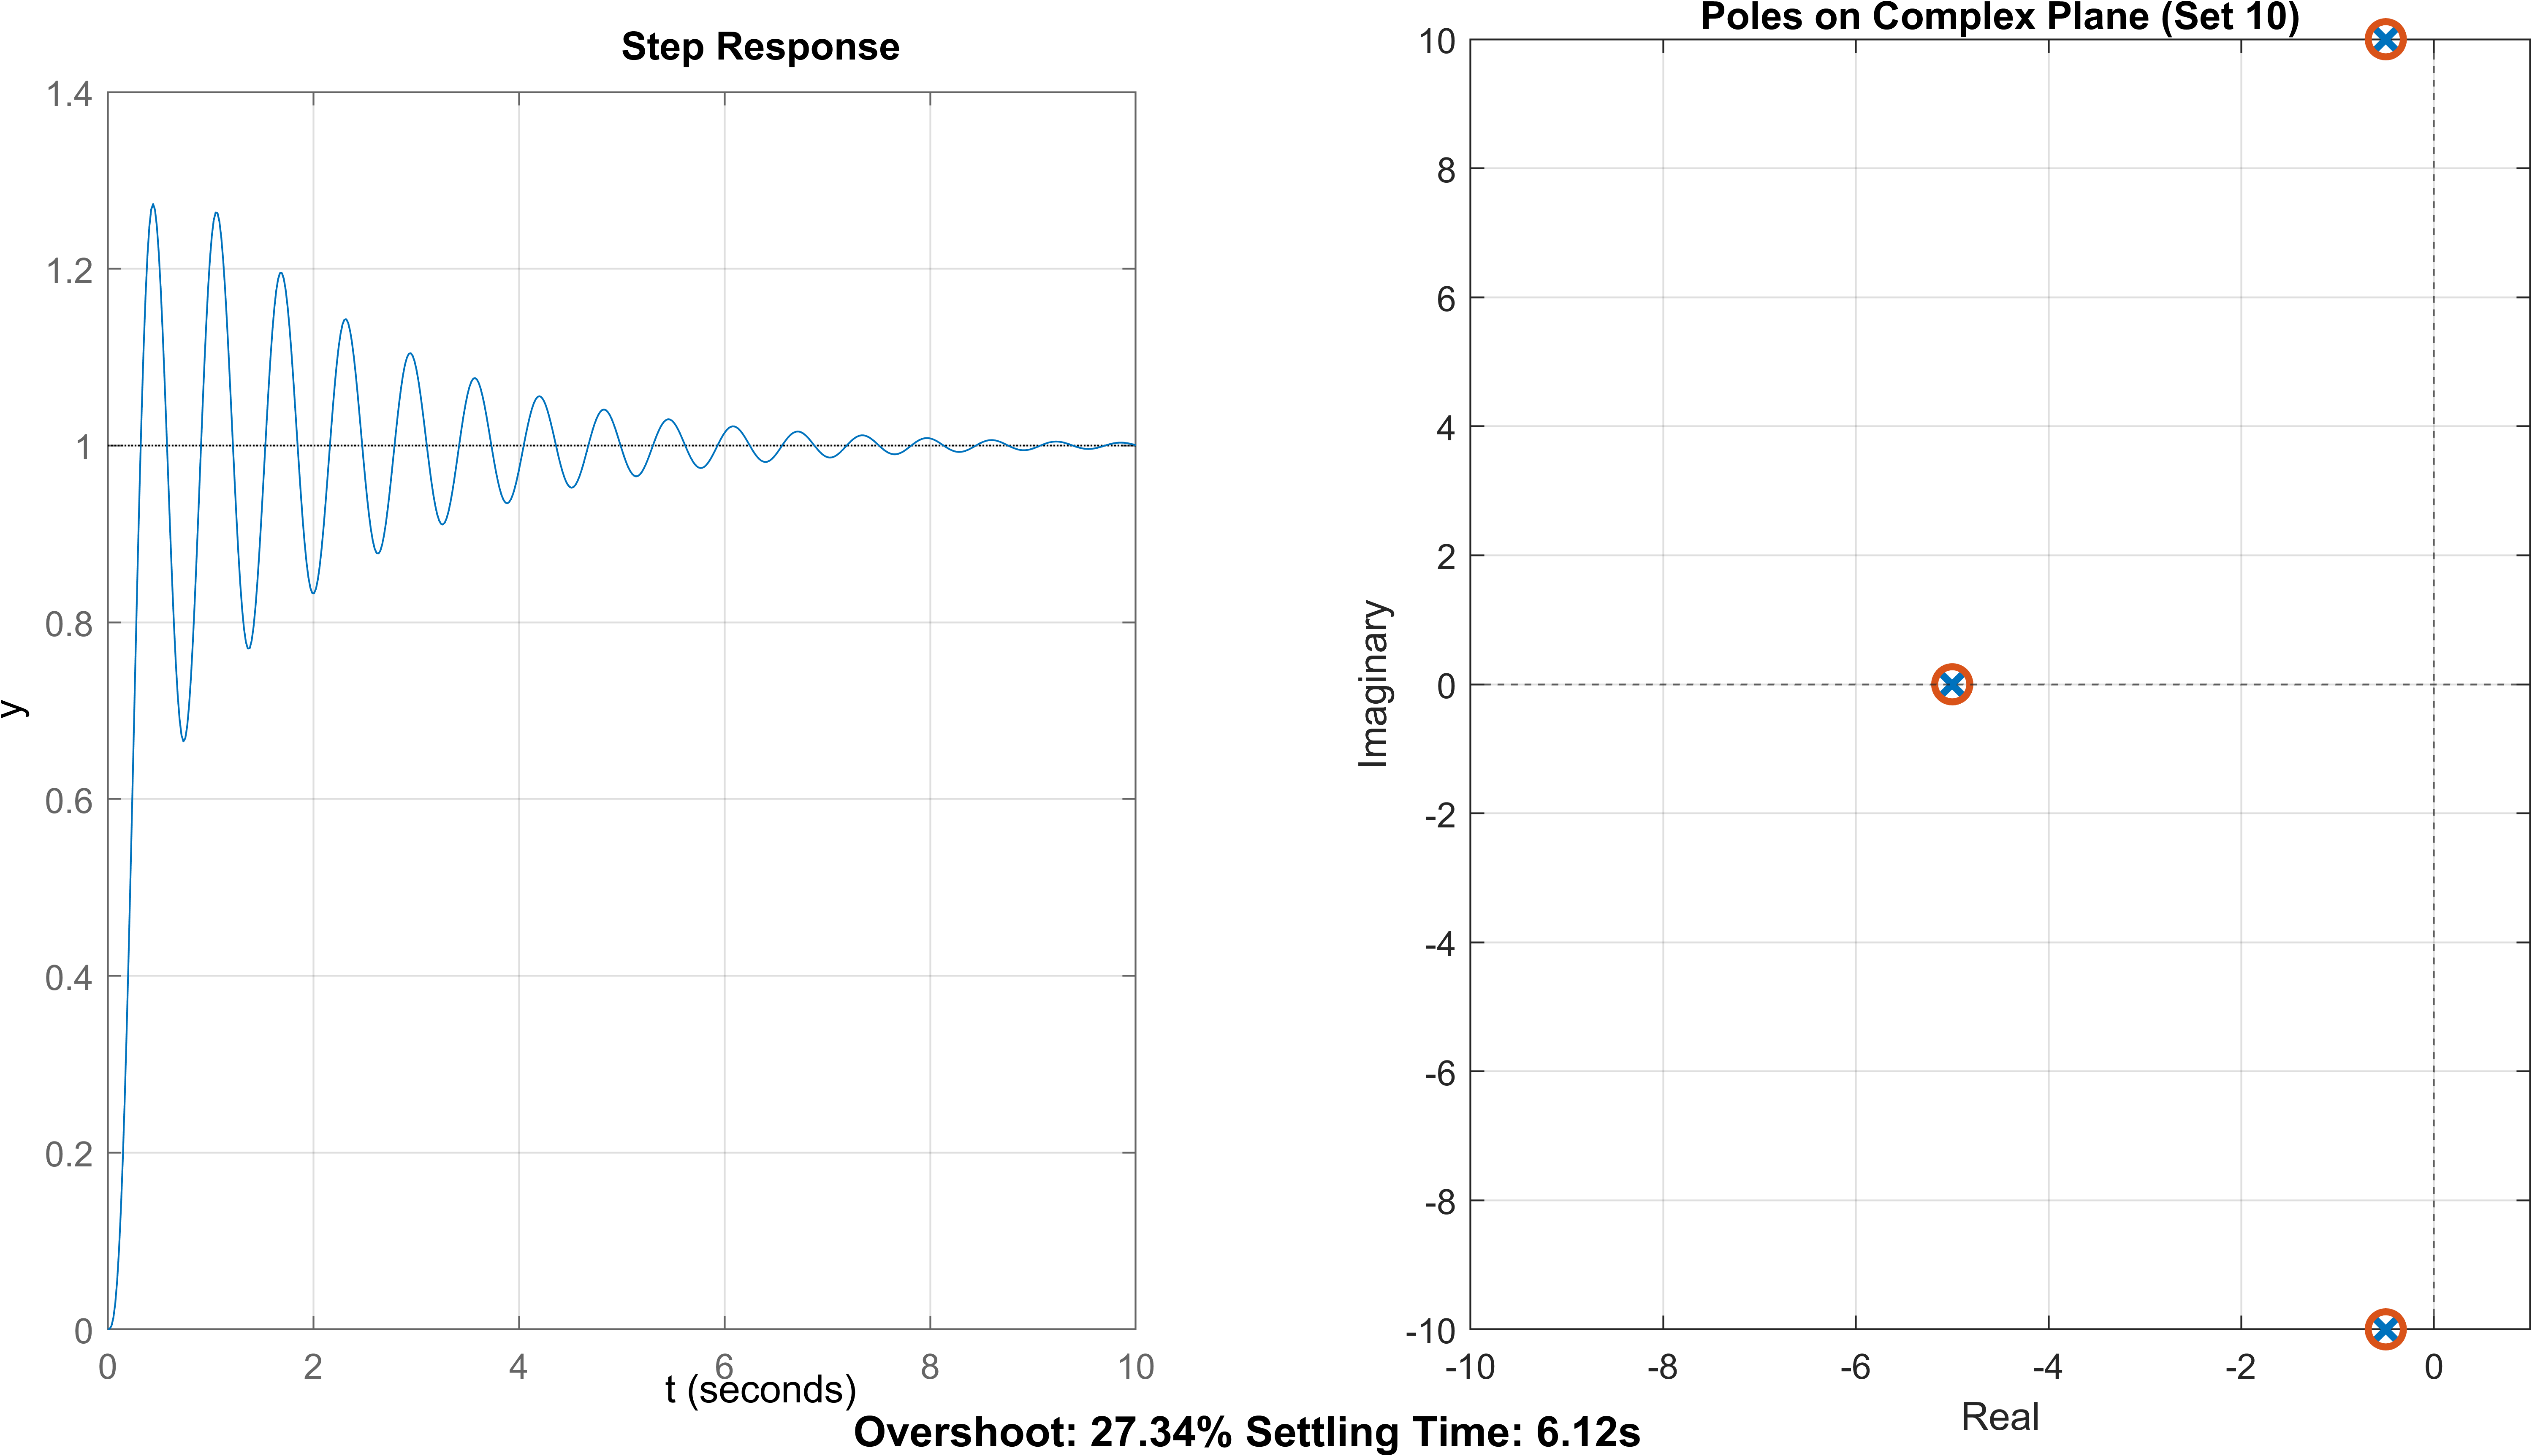
\includegraphics[width=1\textwidth, trim={0cm 0cm 0cm 0cm}]{../images/4_10.png}
    \caption{$\lambda_1 = -0.5+ 10i, \lambda_2 = -0.5 - 10i, \lambda_3 = -5$}
\end{figure}

Из графиков видно, что при увеличении вещественной части полюсов время переходного процесса уменьшается.
В случаях без мнимой части перерегулирование равно нулю, так как переходный процесс не имеет колебаний.
Наличие полюсов с вещественной частью меньше -1 приводит к увеличению переходного процесса. Мнимая часть
полюсов влияет на колебательность переходного процесса. Чем больше мнимая часть, тем больше колебаний.
При этом при умеренных значениях мнимой части переходный процесс становится более быстрым без перерегулирования.
\endinput